\documentclass[abstract=on,10pt,a4paper,bibliography=totocnumbered]{scrartcl}
\usepackage[utf8]{inputenc}
\usepackage[english]{babel}
\usepackage{amsmath}
\usepackage{colortbl}
\usepackage{amsfonts}
\usepackage{amssymb}
\usepackage{graphicx}
\usepackage{enumerate}
\usepackage{epstopdf}
\usepackage[onehalfspacing]{setspace}
\usepackage[paper=a4paper,left=30mm,right=30mm,top=20mm,bottom=25mm]{geometry}
\usepackage[round]{natbib}
\usepackage[hidelinks]{hyperref}
\usepackage[nameinlink]{cleveref}
\usepackage{multirow}
\usepackage{booktabs}
\usepackage[labelfont=bf]{caption}
\usepackage{footnote}
\usepackage{tabularx}
\usepackage{gensymb}
\usepackage{todonotes}
\usepackage{tikz}
\usepackage{subcaption}
\usepackage{varwidth}
% \usepackage[nomarkers,figuresonly]{endfloat}
\usepackage{csvsimple}
\usepackage{arydshln}
\usepackage{titlesec}

% Define a new command to create a number inside a circle (for plots)
\newcommand*\circled[1]{\tikz[baseline=(char.base)]{
            \node[shape=circle,draw,inner sep=1pt] (char) {#1};}}

% Creating some TikZ styles
\tikzset{
  nonterminal/.style = {rectangle
    , minimum size = 6mm
    , very thick
    , draw = black!
  }
}

% Increase the space between two rows in tables
\renewcommand{\arraystretch}{1.2}

% Changing the style of captions in figures etc.
\captionsetup{labelfont=bf, format=plain, font=small}

% Adjust the distance between title and paragraph
\RedeclareSectionCommand[
  beforeskip=-.5\baselineskip,
  afterskip=.5\baselineskip]{subsection}
\RedeclareSectionCommand[
  beforeskip=-.25\baselineskip,
  afterskip=.25\baselineskip]{subsubsection}

\doublespacing
\begin{document}
\pagenumbering{gobble}
\bibliographystyle{apalike}

\begin{titlepage}

% Define a new command to produce a horizontal line
\newcommand{\HRule}{\rule{\linewidth}{0.5mm}}

% Center everything on the page
\center

%------------------------------------------------------------------------------
%	HEADING SECTIONS
%------------------------------------------------------------------------------

% Name of your university/college
\textsc{\LARGE  }\\[1.5cm]

% Major heading
\textsc{\Large Department of Evolutionary Biology and Environmental
Studies}\\[0.5cm]

% Minor heading
\textsc{\large Master's Thesis}\\[0.5cm]

%------------------------------------------------------------------------------
%	TITLE SECTION
%------------------------------------------------------------------------------
\doublespacing
\HRule \\[0.4cm]

% Title of the document
{\textsc{ \LARGE Running Wild: Movement Corridors of Dispersing African Wild
Dogs (\textit{Lycaon pictus}) in the Kavango-Zambezi Transfrontier Conservation
Area}}\\[0.4cm]

\HRule \\[1.5cm]
\singlespacing

%------------------------------------------------------------------------------
%	AUTHOR SECTION
%------------------------------------------------------------------------------

\begin{minipage}{0.4\textwidth}
\begin{flushleft} \large

% Main author
\emph{Author:}\\
David D. Hofmann\\
david.hofmann2@uzh.ch\\
12-728-846

\end{flushleft}
\end{minipage}
~
\begin{minipage}{0.4\textwidth}
\begin{flushright} \large

% Supervisors
\emph{Supervisors:} \\
Dominik Behr\\
Ph.D. Gabriele Cozzi\\
Prof. Arpat Ozgul

\end{flushright}
\end{minipage}\\[2cm]

%------------------------------------------------------------------------------
%	DATE SECTION
%------------------------------------------------------------------------------

% Today's date
{\large \today}\\[5cm]

%------------------------------------------------------------------------------
%	LOGO SECTION
%------------------------------------------------------------------------------

% Logo of the university
\includegraphics{UZHVector.eps}\\[1cm]

%------------------------------------------------------------------------------

% Fill the rest of the page with whitespace
\vfill

\end{titlepage}

\begin{abstract}
The African wild dog \textit{(Lycaon pictus)} is an endangered species that
currently only survives in a few scattered subpopulations in Sub-Saharan Africa.
Long-term viability of the species thus requires the identification and
preservation of key dispersal corridors that connect such subpopulations. We
collected GPS data of 16 dispersing coalitions originating from a free-ranging
population in northern Botswana and used integrated step selection analysis to
create a permeability surface spanning over the entire Kavango-Zambezi
Transfrontier Conservation Area (KAZA-TFCA), the largest transboundary
conservation area on earth. Based on our permeability surface, we calculated
least-cost paths and least-cost corridors between selected locations within the
KAZA-TFCA. Our results show that dispersal corridors typically run through open
shrubs/grassland, and in the vicinity of water. Corridors rarely cross
waterbodies, areas with high human presence, or areas densely vegetated by
trees. Several dispersal corridors meet in the Linyanti-Chobe ecosystem, which
highlights the importance of northern Botswana for the conservation of this
charismatic species.
\end{abstract}
\newpage

\onehalfspacing
\tableofcontents
\doublespacing
\newpage

\pagenumbering{arabic}

\section{Introduction}
% Importance of Connectivity
Successful conservation of spatially fragmented subpopulations requires to
assess connectivity of habitats occupied by these subpopulations. In this
context, connectivity describes the degree to which the landscape facilitates or
impedes movement of the focal species between habitat patches
\citep{Taylor.1993, Clobert.2012}. Thus, connectivity is a prerequisite for
dispersal, which in turn promotes genetic exchange, reinforcement of small
populations, and colonization or recolonization of unoccupied habitats
\citep{Brown.1977, Hanski.1998, MacArthur.2001, Frankham.2002, Leigh.2012}. All
of these processes crucially contribute to the long-term viability of numerous
species, therefore emphasizing the importance of connectivity. However,
increasing anthropogenic pressure and ongoing loss and fragmentation of valuable
habitats erode connectivity on a worldwide scale \citep{Fahrig.2003,
Barnosky.2012}. As a result, management actions for the conservation of
endangered species increasingly aim to restore connectivity through the
identification and preservation of key movement corridors that link isolated
habitats \citep{Fahrig.2003, Heller.2009}. An unprecedented instance of an
initiative to restore connectivity on a large scale is the Kavango-Zambezi
Transfrontier Conservation Area (KAZA-TFCA), which traverses five African
countries and spans over 520,000km\textsuperscript{2}. While the primary purpose
of the KAZA-TFCA is to facilitate the migration of elephants across large
landscapes, numerous other wide-ranging species will likely benefit from its
planned protectorates too. Nevertheless, the extent to which such initiatives
are beneficial to certain species is rarely assessed, leaving open their true
impact on connectivity.

% African wild dogs
One of the species for which the degree to which it will benefit from the
KAZA-TFCA remains unknown is the African wild dog (\textit{Lycaon pictus}), a
keystone predator and flagship species for conservation efforts in the KAZA-TFCA
\citep{VanDerMeer.2016}. While once present across the entire Sub-Saharan
continent, the species has been widely extirpated through human persecution,
habitat destruction and disease outbreaks. As a result, the African wild dog has
become Africa's most endangered large carnivore that currently only survives in
small, spatially scattered subpopulations (see \Cref{StudyArea}a,
\cite{Woodroffe.2012}). Within these subpopulations, wild dogs form cooperative
breeding groups of up to thirty individuals in which a single dominant pair
monopolizes the majority of reproduction \citep{Frame.1979, Fuller.1992,
Creel.2002}, while subordinates of both sexes help to feed newborn pups
\citep{Malcolm.1982}. After reaching 15 months of age, male and female offspring
disperse from their natal pack in same-sex coalitions and search for unrelated
mates and a suitable territory to settle (\citeauthor{McNutt.1996}, 1996;
\citeauthor{Behr.2019}, unpublished). During such dispersal events, wild dogs
cover vast distances, sometimes crossing perilous areas that are strongly
influenced by humans (\citeauthor{DaviesMostert.2012}, 2012;
\citeauthor{Masenga.2016}, 2016; \citeauthor{Cozzi.2019}, in review). Despite
the importance of dispersal for the remaining wild dog subpopulations, little is
known about the movement corridors of dispersing individuals and connectivity
between subpopulations in the KAZA-TFCA in general.

% Connectivity Assessment
In recent years, there has been a growing body of literature that uses animal
movement data to identify movement corridors and thereby assess connectivity on
large scales \citep{Chetkiewicz.2006}. Revelation of potential movement
corridors between selected locations traditionally relies on the estimation of a
permeability surface (elsewhere referred to as resistance surface when
inverted), which depicts the ease or willingness at which the focal species
traverses a specific landscape. Latest and very powerful empirical methods to
predict permeability based on observed movements include \textit{resource
selection functions} (RSF, \cite{Boyce.2002}), \textit{step selection functions}
(SSF, \cite{Fortin.2005}) and \textit{path selection functions} (PSF,
\cite{Cushman.2010}). All methods have in common that they infer habitat
preferences of the focal species by comparing environmental covariates at
visited locations to environmental covariates at randomly selected locations
that are deemed available but presumably unused by the animal. Based on inferred
habitat preferences, the methods further assume that habitats preferred by the
focal species provide high permeability, whereas avoided habitats provide low
permeability. Regardless of the method chosen (i.e. RSF, SSF, or PSF), all
approaches require adequate relocation data that is representative for the
process being studied.

% Behavioral Modes
For connectivity studies in particular, the behavioral mode of the animal (e.g.
resident, dispersing) during data collection should be considered when
estimating landscape permeability and assessing movement corridors. However, few
studies have partitioned their movement data according to behavioral mode
\citep{Wilson.2012, Vasudev.2015}. As a consequence, most researchers estimated
permeability for dispersing individuals as if they had the same preferences as
resident individuals. This is a rather disputed assumption and recent research
suggests that such an approach seriously reduces the power to reveal meaningful
movement corridors \citep{Killeen.2014}. For instance, \cite{Elliot.2014}
demonstrated marked differences in predicted permeability surfaces for
dispersing lions in the KAZA-TFCA depending on whether permeability was assessed
using data collected during residence or dispersal. \cite{Jackson.2016} made
similar observations for African wild dogs and revealed higher permeability for
dispersers than for residents. Moreover, \cite{Abrahms.2017} found a
significantly greater overlap between predicted and observed corridors for three
dispersing wild dogs when predictions were based on information collected during
wild dog activity, rather then when ignoring the behavioral mode. Overall,
predicted movement corridors vastly differed depending on the type of data that
was being used \citep{Elliot.2014, Jackson.2016, Abrahms.2017}. Unfortunately,
data of dispersing wild dogs remains scarce and is collected opportunistically
at best \citep{DaviesMostert.2012, Masenga.2016, Jackson.2016, Abrahms.2017}.
For instance, the dispersers reported in \cite{DaviesMostert.2012} were not
fitted with global positioning system (GPS) collars, which is why the
researchers only recorded straight line dispersal-distances.
\cite{Masenga.2016}, on the other hand, were able to collect proper GPS data,
yet only on two dispersers. Furthermore, \cite{Jackson.2016} based their work on
occasional wild dog sightings and their distinction between residents and
dispersers was based purely on group size, assuming that any group with fewer
than nine members was dispersing. Finally, \cite{Abrahms.2017} used GPS
relocation data of resident individuals during phases of activity rather than
during true dispersal. In summary, none of these studies systematically
monitored dispersing individuals, which is likely owed to technological and
logistic limitations when monitoring such an elusive and wide-ranging species
\citep{Nathan.2001, Tesson.2013}. Yet, a better understanding of how the
landscape impedes or facilitates movement of dispersers is vital for improving
our understanding of connectivity and for conservation of the species in
general.

% Research Goal
Our study therefore had two aims: (1) to estimate landscape permeability for
dispersing wild dogs, and subsequently use this information to (2) assess
connectivity by revealing key dispersal corridors within the entire extent of
the KAZA-TFCA. For this purpose, we collected GPS data of 16 dispersing
coalitions originating from a free-ranging population of wild dogs in the
eastern section of the Okavango Delta in Botswana. We highlight key dispersal
corridors that provide connectivity between already established protected areas
within the KAZA-TFCA and we reveal potentially important dispersal corridors
outside the planned protectorates of the KAZA-TFCA. Our results have important
implications for the conservation and management of the endangered African wild
dog.

\newpage
\section{Methods}
\subsection{Study Area}
% Core Study Area
For the purpose of this study we differentiated between a \textit{core study
area}, where all dispersers originated from, and an \textit{extended study
area}, for which we conducted the connectivity analysis. The \textit{core study
area} was located in the eastern section of the Okavango Delta in northern
Botswana (\Cref{StudyArea}b, centered at -19\degree 25'30''S, 23\degree
37'30''E; elevation ca. 950m) and comprised parts of the Moremi Game Reserve and
adjacent wildlife management areas. The Okavango Delta is considered to be one
of the main strongholds of African wild dogs in southern Africa and likely acts
as a source for the recolonization of surrounding habitats
\citep{Woodroffe.2012, Cozzi.2013}. The Okavango Delta represents the earth's
largest inland delta and is characterized by diverse habitats, ranging from
permanent river systems, mopane woodland and acacia forests, to open grasslands
and seasonal swamps \citep{Broekhuis.2013}. Rainfall is periodic and lasts from
November to March, whereas the rest of the year remains dry \citep{McNutt.1996}.
Flooding of the delta greatly changes depending on the season and drastically
affects surrounding landscapes (see \Cref{FloodPulse} in
\Cref{Appendix:FloodPulse} for an illustration of a typical flood pulse). During
maximum extent, the delta becomes a patchy conglomerate of swamps, open water,
and islands. Because rainfalls only slowly descent from their catchment areas in
southern Angola into the Okavango Delta, the flood usually peaks at the height
of the dry season between August and September \citep{Wolski.2017}. Most of the
Okavango Delta's unique basin is under protection, such that human influence in
our core study area was mainly restricted to the surroundings of Maun and the
smaller villages of Khwai, Mababe, and Sankuyo.

% Large Study Area
Our \textit{extended study area} was confined by the extent of the KAZA-TFCA
(\Cref{StudyArea}a, centered at -17\degree 13'9''S, 23\degree 56'4''E; elevation
ca. 1,030m), which lies in the basins of the Okavango and Zambezi rivers and
embraces parts of Angola, Botswana, Namibia, Zimbabwe, and Zambia. With a total
area of over 520,000km\textsuperscript{2} the KAZA-TFCA contains several already
existing national parks (NPs) and other protected areas, and will eventually
become earth's largest transboundary conservation area. Since we considered the
entire rectangular extent of the KAZA-TFCA, our extended study area encompassed
a total of over 1.3 Mio km\textsuperscript{2}. Similar to our core study area,
the extended study area hosts a conglomerate of various landscapes, including
savanna, grassland, and dry or moist woodland patches. Furthermore, the
KAZA-TFCA encloses several wild dog subpopulations  that still reside in
Namibia, Botswana, and Zimbabwe (\Cref{StudyArea}a, \cite{Woodroffe.2012}).
Despite 36 NPs and numerous other protected areas, there is considerable human
influence in some regions of the KAZA-TFCA originating from farms, high human
density, and road traffic.

\begin{figure}[h]
  \begin{center}
    \begin{tikzpicture}
        \node[anchor=south west,inner sep=0] (image) at (0,0,0) {
        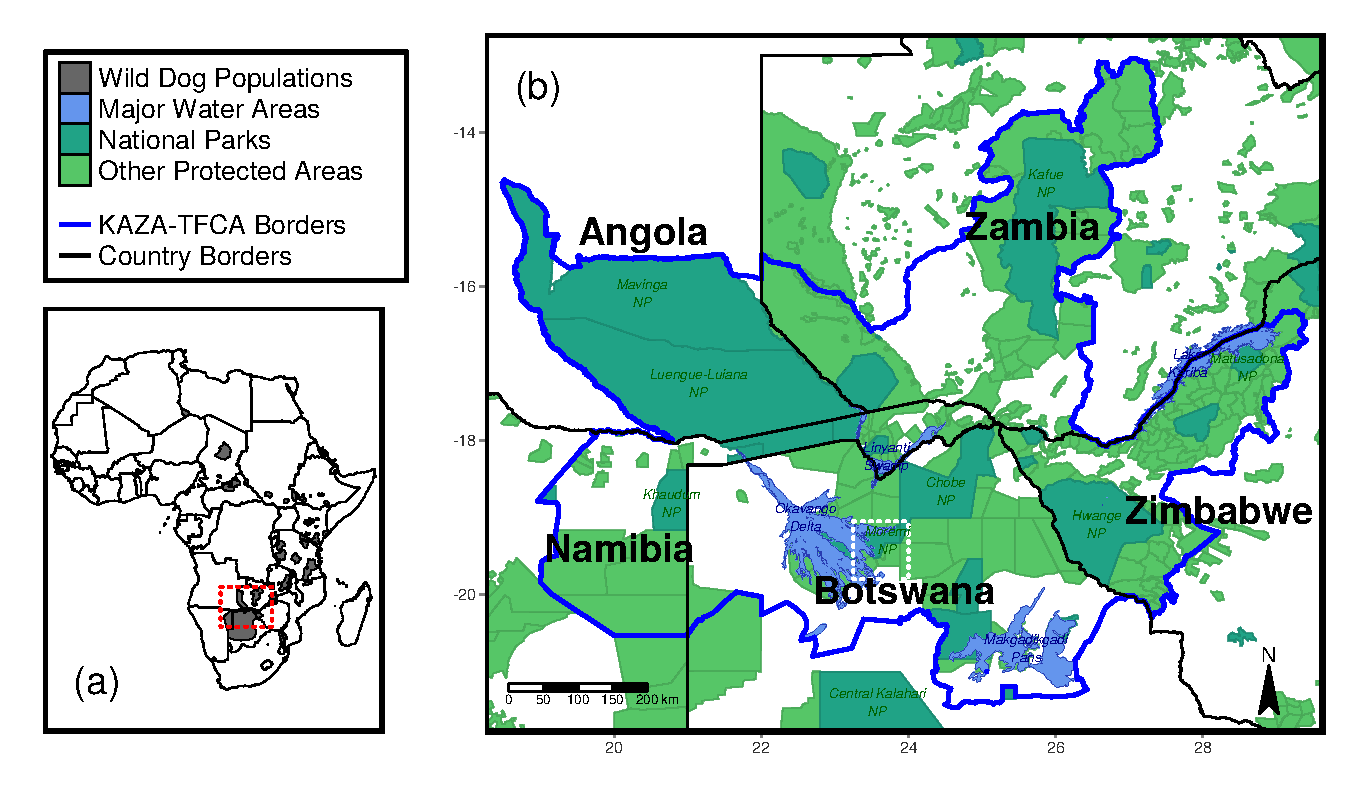
\includegraphics[width=\textwidth]{99_StudyArea.pdf}
        };
        \begin{scope}[x={(image.south east)},y={(image.north west)}]
            % % next four lines will help you to locate the point needed by forming a grid.
            % % comment these four lines in the final picture.
            % \draw[help lines,xstep=.1,ystep=.1] (0,0) grid (1,1);
            % \draw[help lines,xstep=.05,ystep=.05] (0,0) grid (1,1);
            % \foreach \x in {0,1,...,9} { \node [anchor=north] at (\x/10,0) {0.\x}; }
            % \foreach \y in {0,1,...,9} { \node [anchor=east] at (0,\y/10) {0.\y};}
            % % upto here
            \draw[black] (0.202, 0.255) -- (0.36, 0.955);
            \draw[black] (0.202, 0.205) -- (0.36, 0.070);
        \end{scope}
    \end{tikzpicture}
    \caption{Overview of our study area. (a) The red rectangle depicts our
    \textit{extended study area}, which was confined by the extent of the
    KAZA-TFCA. Purple areas indicate remaining wild dog populations according to
    the IUCN \citep{Woodroffe.2012}. (b) The orange rectangle illustrates our
    \textit{core study area}, from which all dispersers departed. Yellow lines
    depict all dispersal trajectories that were recorded between the years 2011
    and 2019. Since game reserves in Botswana virtually serve the same purpose as
    National Parks, we will use the terms interchangeably for this region.}
    \label{StudyArea}
  \end{center}
\end{figure}

\subsection{GPS Relocation Data}
% Collection
We collected GPS relocation data of 16 wild dog coalitions (i.e. 7 female and 9
male coalitions) that dispersed from the core study area between 2011 and 2019.
Potential dispersing individuals were immobilized according to protocols
described in \cite{Osofsky.1996} and fitted with GPS/Satellite radio collars
(\textit{Vertex Lite; Vectronic Aerospace GmbH, Berlin}) while they were still
with their natal pack. All required procedures were undertaken and supervised by
a Botswana-registered wildlife veterinarian. Immobilized individuals were
monitored and all were observed to successfully re-join their packs within one
hour after immobilization. GPS collars were programmed to record and transmit
GPS relocations via Iridium satellite system to a base station. The system thus
allowed remote-tracking of collared individuals, even where field conditions
were prohibitive or dispersal trajectories crossed international borders.
Because we were mainly interested in recording dispersal trajectories,
relocations were collected only every 24 hours during residence, but every 4
hours during dispersal. Dispersal and residence were strictly distinguished
using a combination of net squared displacement \citep{Borger.2012}, visual
inspection of trajectories, and observations of pack constellations in the field
(for details see \citeauthor{Cozzi.2019}, in review). Dispersal was deemed to
have started when an individual left its natal home range, and continued until
the individual formed a new pack or exhibited signs of resident behavior. Some
dispersers undertook exploratory movements prior to dispersal. Such movements
have been observed in other species as well and are reported to be very similar
to true dispersal \citep{Killeen.2014}. We therefore classified exploratory
movements as dispersal too. We did not attempt to distinguish sex in our
analysis, as previous research found little differences between males and
females during dispersal (\citeauthor{Woodroffe.2019}, 2019;
\citeauthor{Cozzi.2019}, in review). In total, we collected 4,691 GPS
relocations during dispersal (see \Cref{Trajectories}). On average, dispersal
events included three individuals (min = 1, max = 7), lasted for 41 days (min =
7, max = 133), and covered a mean cumulative distance of 370km (min = 105, max =
610). Detailed descriptions of the dispersal events can be found in
\citeauthor{Cozzi.2019} (in review). Although our final sample size of 16
dispersers was relatively small, we consider this an exceptional number for such
an endangered and elusive species.

\begin{figure}[h]
  \begin{center}
    \includegraphics[width = \textwidth]{99_Trajectories.pdf}
    \caption{Illustration of the dispersal trajectories that we recorded. Each
    color represents a different dispersal coalition. All coalitions departed
    from our core study area, which is indicated by the white square. The
    coalition dispersing towards the far east of the map covered over 360km in
    under 10 days.}
    \label{Trajectories}
  \end{center}
\end{figure}

\subsection{Covariates}
% General stuff
We used a set of geo-referenced covariates to investigate movement and habitat
preferences of dispersing wild dogs (see \Cref{Covariates}). Covariates fell
into one of the three categories \textit{land cover}, \textit{protection
status}, and \textit{human influence}. For each category we obtained spatial
raster layers from freely available online services or from remote sensed
satellite imagery. To ensure a consistent resolution (i.e. cell-size or grain)
across covariates, all layers were coarsened or interpolated to match a
resolution of 250m x 250m. Processing and manipulation of data, as well as all
spatial and statistical analyses were performed in R, version 3.6.1
\citep{R.2019}.

\begin{figure}[h]
  \begin{center}
    \includegraphics[width = \textwidth]{99_Covariates.pdf}
    \caption{Overview of covariates that we used in our models. Although all
    covariates were prepared for the extended study area, we present only an
    extract to maximize visibility. The white square in each plot depicts our
    core study area. (a) Averaged layer of all binary maps of water and dryland
    that we acquired using our remote sensing algorithm. (b) Percentage cover of
    trees. (c) Percentage cover of shrubs/grassland. Note that anything not
    covered by trees or shrubs/grassland was deemed to be bareland. (d)
    Protection status according to the Peace Parks Foundation. (e) Human
    influence proxy, including human density, farms, and roads. (f) Distance to
    nearest road (white lines depict actual roads).}
    \label{Covariates}
  \end{center}
\end{figure}

\subsubsection{Land Cover}
% Overview
Land cover was represented by four layers: (1) a binary layer distinguishing
water and dryland, and (2) three continuous layers showing the percentage cover
by different vegetation types, together adding up to 100\%.

% Dynamic Watermapping
(1) For the purpose of this study, water included open waters, rivers, wetlands,
and swamps, whereas anything else was presumed to be dryland. Because flooding
of the Okavango Delta is highly variable, we decided to map the flood
dynamically for the extent shown in \Cref{Floodmapping}. To create dynamic
``floodmaps'', we applied an algorithm that was originally designed by the
\textit{Okavango Research Institute} (ORI) and is explained in detail by
\cite{Wolski.2017}. However, we rewrote and slightly amended the original Python
code in R and thus describe the underlying principles again and especially
indicate the discrepancies to the original algorithm.

\begin{figure}[h]
  \begin{center}
    \includegraphics[width = \textwidth]{99_Floodmapping.pdf}
    \caption{Figures describing the floodmapping algorithm. (a) The colored
    polygons indicate permanent waters and permanent dryland. Below these
    polygons we extracted reflectance values of MODIS Terra Band 7 and used
    their repsective medians to calculate a classification threshold. (b)
    Example of a classified MODIS Terra Band 7 image after application of the
    threshold.}
    \label{Floodmapping}
  \end{center}
\end{figure}

% Algorithm
To implement the algorithm, we defined two sets of polygons located in the
region of the Okavango Delta (see \Cref{Floodmapping}). The first set consisted
of areas known to be permanent dryland, whereas the second set consisted of
permanent waters. Since we were unable to retrieve the original polygons used in
\cite{Wolski.2017}, we geo-referenced one of their illustrations and traced the
polygons there. After recreation of the polygons, we used the R-package
\textit{getSpatialData} \citep{Schwalb.2018} to download and pre-process all
relatively cloud-free MODIS Terra images (MCD43A4, \cite{Schaaf.2015}) available
for the period of our dispersal events. Assessment of cloud cover was based on
visual inspection of MODIS images on ORI's website \citep{ORI.2019}. The MCD43A4
MODIS product is particularly useful for dynamic floodmapping because it is
updated with new composite images every 8th day \citep{Wolski.2017}. After
download, we classified each MODIS image into a binary map of water (flood) and
dryland using a threshold that was identified as follows. First, we extracted
all reflectance values of MODIS Terra Band 7 within the water- and
dryland-polygons. Second, we computed histograms of water-reflectances and
dryland-reflectances and empirically verified that reflectances of the two
groups were sufficiently distinct. More specifically, we checked if
superimposing the two histograms resulted in a bimodal plot. This was said to be
achieved if the 99\textsuperscript{th} percentile of water-reflectances did not
severely exceed the 1\textsuperscript{st} percentile of dryland-reflectances
(\(p_{0.99, water} - \frac{10}{255} < p_{0.01, dryland}\)). Third, if peaks were
sufficiently different, we calculated a threshold (\(t\)) using \Cref{EQ1}:

\begin{equation}
\label{EQ1}
t = \widetilde{p}_{water} + 0.3 * (\widetilde{p}_{dryland} -
\widetilde{p}_{water})
\end{equation}

\noindent where \(\widetilde{p}_{water}\) and \(\widetilde{p}_{dryland}\) were
the median reflectances of water and dryland, respectively. We then classified
all pixels of MODIS Terra Band 7 with a value greater than \(t\) as dryland and
all pixels with a value smaller than \(t\) as water.

% Dynamic Wetmask
Importantly, bimodality was not always achieved and in some cases no floodmap
could be calculated. In fact, it appears that non-bimodality caused the ORI
algorithm to fail since the end of 2018, such that no floodmaps have been
generated since then (ORI, personal comm.). We hypothesized that this was caused
by the application of static water-polygons that did not cover permanent waters
correctly anymore. We therefore revised the algorithm and allowed for a more
dynamic polygonization of water. That is, for each MODIS image we calculated new
water-polygons comprising areas that were covered by the flood in 99\% of the
floodmaps from the previous five years. All of the necessary floodmaps from
previous years were kindly provided to us by ORI. Using this slightly amended
approach, we were able to address some of the bimodality issues and to classify
several additional floodmaps for the period of our study. Because MODIS Terra
Band 7 had a resolution of 500m x 500m, we interpolated all maps to 250m x 250m.

% Validation
To validate and compare the performance of our own algorithm to the original
ORI-algorithm, we randomly sampled 48 dates for which ORI prepared classified
images. To make sure that months were equally represented in the sampled dates,
we employed stratified sampling based on months (regardless of the year) and
randomly sampled four maps for each month. For the sampled dates we downloaded
and classified MODIS Terra Band 7 images and compared our classified images to
those provided by ORI (\Cref{FloodmappingValidation}). For each pair of maps we
created a difference map indicating false positives and false negatives and
computed the relative number of wrongly classified pixels. We achieved an
overall accuracy of 97\%, which presumably is an underestimate of the true
performance, as we introduced some errors when resampling the ORI-maps to our
reference raster.

\begin{figure}[ht]
  \begin{center}
    \includegraphics[width = \textwidth]{99_FloodmappingValidation.pdf}
    \caption{Validation procedure of our floodmapping algorithm. (a) Classified
    image that was provided to us by ORI. (b) Image for the same date but now
    classified using our own algorithm. (c) Difference image indicating false
    positives and false negatives in our own classification.}
    \label{FloodmappingValidation}
  \end{center}
\end{figure}

% Static Watermap
\noindent While water in the Okavango Delta was mapped dynamically, we used a
static watermap for its surroundings. This static map was based on Globeland's
land cover dataset \citep{Chen.2015}, which contains ten land cover categories.
From the original layer we only retained the categories \textit{wetland} and
\textit{waterbodies} and collectively reclassified them to \textit{water}.
Globeland had an original resolution of 30m x 30m, so we coarsened the layer to
250m x 250m using the mode of each 250m x 250m cell. Lastly, we improved river
representation using the MERIT Hydro dataset \citep{Yamazaki.2019}, from which
we added all rivers with a width of over 10m to our watermaps. The entire
process resulted in several hundred watermaps, of which 72 represented the
closest watermap to one of our GPS relocations.

(2) The three vegetation layers that we used in addition to the water/dryland
maps were derived from the MODIS Terra Vegetation Continuous Fields dataset
(MOD44B, \cite{Dimiceli.2015}). Combined, the layers added up to 100\% and
depicted the percentage cover of tree-vegetation (henceforth trees),
non-tree-vegetation (henceforth shrubs/grassland), and non-vegetated (henceforth
bareland). Since we wanted to make sure that areas covered by the flood would
get 0\% vegetation cover (i.e. 100\% bareland cover), we used our floodmap that
aligned with the creation date of the layers (30 March 2017) and set all flooded
pixels to 100\% bareland. The MODIS vegetation layers had a resolution of 250m x
250m, so we did not need to coarsen or interpolate them.

\subsubsection{Protection Status}
To assess whether dispersers preferred protected over unprotected (pastoral)
regions, we derived a binary layer separating the two categories. Corresponding
data on protection status was downloaded in shapefile format from the Peace
Parks Foundation \citep{PeaceParks.2019}. We simplified original categories to a
binary classification of protected and pastoral areas (see
\Cref{Reclassification} in \Cref{Appendix:Reclassification}). Protected areas
mainly included forest reserves, game reserves, wildlife management areas, and
NPs, whereas everything not covered by such categories was considered to be
pastoral area. Finally, we rasterized the two categories onto a binary raster (1
= protected, 0 = pastoral) with a resolution of 250m x 250m.

\subsubsection{Human Influence}
We depicted human influence in our study area using a proxy that incorporated
anthropogenic pressures arising from (1) human density, (2) farming, and (3)
roads. Previous research revealed that veterinary fences have no influence on
wild dog movement, so we did not include them in our analysis
\citep{Cozzi.2013b}.

% Human Density
(1) Spatial human density estimates were obtained through Facebook's 30m x 30m
high resolution population density dataset \citep{Facebook.2019}. The dataset
contained some human density that arised from lodges and other touristic
activities that we did not want to depict as human pressures, so we manually
removed such regions from the data. The resulting layer was coarsened to 250m x
250m by summing up human densities within 250m x 250m cells.

% Farming
(2) Information on agricultural activities was sourced from the Globeland
\citep{Chen.2015} and Cropland \citep{Xiong.2017} land cover datasets, from
which we only retained pixels that were classified as either \textit{cultivated
land} or \textit{croplands}. Both layers had a resolution of 30m x 30m and were
coarsened to 250m x 250m by summing up values within 250m x 250m cells. The
layers were then merged into a single binary layer depicting presence (= 1) or
absence (= 0) of farms within 250m x 250m cells.

% Roads
(3) Geo-referenced data on roads was downloaded in shapefile format from Open
Street Map \citep{OpenStreetMap.2019}. We omitted minor roads and only retained
main tar roads and trunks belonging to the biggest four categories (see
\Cref{Appendix:RoadCategories}). Finally, we rasterized roads and trunks onto a
binary raster (1 = roads, 0 = no roads) with 250m x 250m resolution.

To calculate a single proxy of human influence, we added up the layers
describing \textit{human density} (continuous), \textit{farming} (binary), and
\textit{roads} (binary). To reduce the influence of outliers, added values
were limited to a maximum of 50, which visually resulted in a good balance
between high and low anthropogenic influence and was therefore considered
appropriate for our analysis. To render the fact that humans influence their
surroundings beyond their presence, we followed \cite{Elliot.2014} and applied
to each pixel a 5km spatial buffer within which we summed up and log-transformed
human-influence values.

\subsection{Permeability Model}
\label{Modeling}
% Explanation of iSSF and Extraction
To parameterize a permeability model and thereby investigate movement and
habitat preferences of dispersing African wild dogs, we used an integrated step
selection function (iSSF, \cite{Avgar.2016}). In the iSSF framework, covariates
along realized steps are contrasted with covariates along random steps that the
animal could have taken, but decided not to. A step is here defined as the
connecting line between two consecutive GPS relocations \citep{Turchin.1998}. In
contrast to regular SSFs, iSSFs require to include movement metrics as
covariates in the corresponding conditional logistic regression model. Their
inclusion in turn allows simultaneous inference on habitat and movement
preferences, as well as to reduce potential biases in estimated habitat
preferences \citep{Forester.2009, Warton.2013, Avgar.2016}.

In order to conduct an iSSF analysis, we strictly followed published
recommendations described in \cite{Avgar.2016}. We prepared our GPS relocation
data for iSSF-analysis using the R-package \textit{amt} \citep{Amt.2019} and
coerced relocations recorded during dispersal to steps that were regularly
spaced four hours apart (allowing for a minor mismatch of up to 15 minutes).
Steps that were separated by more than four hours (e.g. due to GPS failure) were
omitted from further analysis. Each remaining step was paired with 24 random
steps, generated by sampling turning angles from a uniform distribution
U(\(-\pi, \pi\)) and step lengths from a gamma distribution that was fitted
using realized step lengths (shape = 0.3677, scale = 6,302)). Together, a
realized and its 24 associated random steps formed a stratum and received a
unique identifier. Along realized and random steps we extracted environmental
covariates as listed in \Cref{ExtractedCovars}. For continuous covariates we
calculated the average value along the step, for binary covariates the
percentage cover along the step. Since our floodmaps were dynamic, we extracted
values from the floodmap that was closest in date to the actual step. We further
derived a binary variable indicating whether or not a step crossed a road and we
identified the average distance of the step to the nearest source of water or
road. The values for \textit{DistanceToRoads} and \textit{DistanceToWater} were
square-rooted to simulate a decreasing marginal impact of distance. Extracted
covariates were standardized to a mean of zero and a standard deviation of one
using a z-score transformation. We also screened covariates for correlation
using Pearson's Correlation Coefficient. None of the covariates were overly
correlated (\(|r| > 0.6\), \cite{Latham.2011}) and we retained all of them for
modeling. To run a proper iSSF analysis, we also included the movement metrics
\textit{cos(turning angle)} (\(cos(ta\_)\)) and \textit{log(step length)}
(\(log(sl\_)\)) as covariates in our models \citep{Avgar.2016}. The movement
metric \(cos(ta\_\)) served to describe the directionality of a step, as it
transformed the circular measure of (\(-\pi, +\pi\)) into a linear measure (-1,
1), where positive values indicated forward movements, whereas negative values
indicated backwards movements \citep{Turchin.1998}. The movement metric
\(log(sl\_\)), on the other hand, was used as an indicator of the preferred step
length. Since steps were regularly spaced by four hours, \(log(sl\_\)) can also
be interpreted as movement rate.

\begin{table}[h]
  \begin{center}
    \caption{Overview of environmental covariates extracted along steps (see
    \Cref{Sources} in \Cref{Appendix:Sources} for an overview of the sources and
    resampling methods). *The covariates \textit{Water} and \textit{Dryland}
    added up to 100\%, which is why only \textit{Water} was included as
    explanatory variable in our models. The same applied for the group
    \textit{Shrubs/Grassland}, \textit{Trees}, and \textit{Bareland}, where we
    omitted \textit{Bareland} for modeling. Finally, from the group
    \textit{Protected} and \textit{Pastoral}, we only included
    \textit{Protected} in our models.}
    \label{ExtractedCovars}
    \resizebox{\textwidth}{!} {
      \begin{tabular}{lllll}
      \hline
      \textbf{Category} &
        \textbf{Covariate} &
          \textbf{Description} &
            \textbf{Values} \\
              % \textbf{Source(s)} \\
      \midrule
      \multirow{5}{*}{Land Cover}
        & Water
          & Percentage cover of water along step
            & 0-100\%\\
              % & \cite{Chen.2015}, \cite{Schaaf.2015}, \cite{Yamazaki.2019} \\
        & Dryland*
          & Percentage cover of dryland along step
            & 0-100\%\\
              % & Globeland, \cite{Schaaf.2015}, \cite{Yamazaki.2019} \\
        & DistanceToWater
          & Average distance of step to nearest water source
            & \(\geq\) 0m\\
              % & Globeland, \cite{Schaaf.2015}, \cite{Yamazaki.2019} \\
        & Shrubs/Grassland
          & Average non-tree vegetation along step
            & 0-100\%\\
              % & \cite{Dimiceli.2015} \\
        & Trees
          & Average tree-vegetation along step
            & 0-100\%\\
              % & \cite{Dimiceli.2015} \\
        & Bareland*
          & Average non-vegetated area along step
            & 0-100\%\\
              % & \cite{Dimiceli.2015} \\
      \hdashline
      \multirow{2}{*}{Protection Status}
        & Protected
          & Percentage cover of protected area along step
            & 0-100\%\\
              % & \cite{PeaceParks.2019} \\
        & Pastoral*
          & Percentage cover of unprotected area along step
            & 0-100\%\\
              % & \cite{PeaceParks.2019} \\
      \hdashline
      \multirow{3}{*}{Human Influence}
        & HumansBuffer5000
          & Average buffered (5km) human influence along step
            & \(\geq\) 0\\
              % & \cite{Facebook.2019}, \cite{OpenStreetMap.2019}, \cite{Chen.2015}, \cite{Xiong.2017}\\
        & DistanceToRoads
          & Average distance of step to nearest road
            & \(\geq\) 0m\\
              % & \cite{Facebook.2019}, \cite{OpenStreetMap.2019}, \cite{Chen.2015}, \cite{Xiong.2017}\\
        & RoadCrossing
          & Binary value indicating whether a step crossed a road
            & 0, 1\\
              % & \cite{Facebook.2019}, \cite{OpenStreetMap.2019}, \cite{Chen.2015}, \cite{Xiong.2017}\\
      \hline
      \end{tabular}
    }
  \end{center}
\end{table}

% Permeability Model
\noindent We used the iSSF framework and parameterized a permeability model that
further served to predict landscape permeability. This permeability model
operated under the assumption that dispersing wild dogs assigned a selection
score \(w(x)\) of the following exponential form to each realized and random
step:

\begin{equation}
\label{EQ2}
  w(x) = exp(\beta_1 x_1 + \beta_2 x_2 + ... + \beta_n x_n)
\end{equation}

\noindent That is, the selection score \(w(x)\) of a step depended on its
associated covariates (\(x_1, x_2, ..., x_n\)), as well as on the animal's
preferences for these covariates (\(\beta_1, \beta_2, ..., \beta_n\)). The
probability that a step \(i\) was realized \(P(Y_{i} = 1\)) was then contingent
on the step's selection score, as well as on the selection scores of all
alternative steps in the stratum:

\begin{equation}
\label{EQ3}
  P(Y_{i} = 1 | Y_{1} + Y_{2} + ... + Y_{i} = 1) =
  \frac{w(x_{i})}{w(x_{1}) + w(x_{2}) + ... + w(x_{i})}
\end{equation}

% Conditional Logistic Regression Model
\noindent Habitat and movement preferences of interest, i.e. the \(\beta\)'s,
were estimated by comparing realized (scored 1) and random (scored 0) steps in a
conditional logistic regression model \citep{Fortin.2005}. In this model,
positive \(\beta\)-coefficients indicate \textit{selection} of a covariate,
negative \(\beta\)-coefficients \textit{avoidance} of a covariate. Selected
covariates therefore contribute positively to expected landscape permeability,
whereas avoided covariates reduce landscape permeability.

% Mixed Effects Conditional Logistic Regression Model
To deal with multiple individuals, we applied a novel modeling technique for
mixed effects conditional logistic regressions that was recently proposed by
\cite{Muff.2019}. Their approach allowed to include individuals for whom some
covariates did not vary, as well as to model random slopes for each covariate.
We implemented their method using the R-package \textit{glmmTMB}
\citep{Mollie.2017}, where we fixed the variance of the random intercept to an
artificially high value of 10\textsuperscript{12} (for an explanation, see
\cite{Muff.2019}) and used animal ID to model random intercepts and slopes.

% AIC Model Selection
We defined the movement metrics \(cos(ta\_)\) and \(log(sl\_)\) as core
covariates and ran forward model selection based on Akaike's Information
Criterion (AIC, \cite{Burnham.2002}) for environmental covariates. That is, we
started with a univariate model and iteratively increased model complexity upon
reaching a full model. We then ranked models according to AIC, assessed relative
model weights, and identified the most parsimonious model. Due to convergence
issues we were unable to model interactions between environmental covariates.

% Validation
To validate the predictive power of the most parsimonious permeability model, we
ran k-fold cross-validation for case-control studies as described in
\cite{Fortin.2009}. Using 80\% of randomly selected strata, we parameterized a
permeability model and predicted selection scores \(w(x)\) for all steps in the
remaining 20\% of strata. According to predicted selection scores we assigned
ranks 1-25 within each stratum, with rank 1 indicating the highest selection
score. We identified the realized step's rank in each stratum and tallied rank
frequencies for realized steps over all strata. Finally, we carried out a
Spearman-rank correlation analysis between ranks and associated frequencies and
we recorded the correlation coefficient (\(r_{s, realized}\)). We repeated this
procedure 100 times with replacement and computed the mean correlation
coefficient (\(\bar{r}_{s, realized}\)), as well as its 95\% confidence
interval. For comparison, we also repeated the same procedure 100 times assuming
completely randomized preferences. We implemented randomized preferences by
omitting the realized step from each stratum and identifying the rank of a
randomly chosen random step within each stratum (now only ranks 1-24). Again, we
calculated Spearman's rank correlation coefficient (\(r_{s, random}\)), its mean
across repetitions (\(\bar{r}_{s, random}\)), and its 95\% confidence interval.
Ultimately, the validation proofed a significant prediction in case the
confidence intervals of \(\bar{r}_{s, realized}\) and \(\bar{r}_{s, random}\)
did not overlap.

\subsection{Permeability Surface}
We used the most parsimonious permeability model and applied \Cref{EQ2} to
predict a permeability surface over the entire extent of the KAZA-TFCA. Stated
differently, we calculated the selection score \(w(x)\) for each 250m x 250m
pixel covering our extended study area given the pixel's environmental
covariates. Based on the definition of permeability, high selection scores
resulted in high permeability, whereas low selection scores resulted in low
permeability. To reduce the influence of outliers in predicted scores, we
followed \cite{Squires.2013} and curtailed predicted permeabilities between the
1st and 99th percentile of their original values. To predict permeability in the
first place, we needed to collapse all dynamic watermaps into a single layer,
which we achieved by identifying areas that were inundated in at least a quarter
of all our floodmaps. We therefore predicted permeability assuming a relatively
extended flood.

\subsection{Least-Cost Paths \& Least-Cost Corridors}
To identify movement corridors within the extent of KAZA-TFCA, we calculated
least-cost paths (LCPs) and least-cost corridors (LCCs) between source points
located in protectorates of our extended study area \citep{Adriaensen.2003,
Sawyer.2011}. Source points were generated by overlaying the study area with a
regular grid of points, equally spaced 100km apart and located within protected
areas that contiguously covered at least 700km\textsuperscript{2}. The threshold
of 700km\textsuperscript{2} was based on home-range requirements of African wild
dogs reported in \cite{Pomilia.2015} and served to eliminate locations that were
assumed unsuitable for supporting viable wild dog populations. Finally, we
defined centroids as source points for those protectorates with over
700km\textsuperscript{2} that did not get any source points from the regular
grid. In total, we generated 68 source points, which resulted in 2,278 unique
pairwise combinations of source points and therefore 2,278 unique LCPs and LCCs.

LCP analysis between source points was implemented using the R-package
\textit{gdistance} \citep{vanEtten.2018}. The package translated the
permeability surface into a network of nodes and used graph theory, in
particular Dijkstra's algorithm \citep{Dijkstra.1959}, to find shortest
effective distances between source points based on costs of moving from cell to
cell. The package thus required to convert the permeability surface to a
transition layer, where permeability values were translated into transition
probabilities for moving from one cell to another. In our case, the transition
probability of moving between two adjacent cells depended positively on their
averaged permeability. We allowed individuals to move from each cell to the
cell's 8 surrounding neighbors (i.e. Moores neighborhood) and applied a
geographic correction to account for the fact that diagonal neighbors were more
remote than orthogonal neighbors. Because African wild dogs have been observed
to cover massive dispersal distances (\citeauthor{DaviesMostert.2012}, 2012;
\citeauthor{Masenga.2016}, 2016; \citeauthor{Cozzi.2019}, in review), we did not
limit LCPs to a maximal effective cost. After computation, we tallied
overlapping LCPs to identify high-frequency routes.

LCPs are often criticized because they identify single-pixel-wide paths and thus
obliterate potential alternative routes with only marginally higher costs
\citep{Pinto.2009}. Moreover, they implicitly assume that dispersers have
complete knowledge of the landscape and associated movement costs and therefore
always move along the cheapest route \citep{Carroll.2012}. Yet, individuals
rarely use a single optimum path, so that LCPs are often of limited biological
relevance \citep{Pinto.2009, Pullinger.2010}. To address these shortcomings, we
also calculated LCCs \citep{Pinto.2009, Sawyer.2011}, again using the R-package
\textit{gdistance}. In contrast to LCPs, LCCs overcome the
single-pixel-width-issue and reveal additional, slightly suboptimal dispersal
routes. To identify LCCs, we first computed for each source point a cumulative
cost map (see \Cref{LCCExample}), which indicated the total minimal costs
required to get from the respective source point to any other location on the
map. A LCC between two source points was then obtained by adding up their
cumulative cost maps and masking out all cell-values exceeding the lowest
cell-value by more than 5\%. We repeated this procedure for each possible
pairwise combination of source points and thereby identified LCCs between all
source points. The resulting corridor-maps were normalized to a range from zero
to one using \(f(x) = \frac{x - min(x)}{max(x) - min(x)}\) and totaled up into a
single connectivity map.

% \begin{figure}[hbtp]
%   \begin{center}
%     \begin{tikzpicture}
%         \node[anchor=south west,inner sep=0] (image) at (0,0,0) {
%           \begin{minipage}{0.54\textwidth}
%             \begin{center}
%               \includegraphics[width = 0.5\textwidth]
%                 {99_LeastCostPaths(Example1).pdf}\\
%               \includegraphics[width = 1.0\textwidth]
%                 {99_LeastCostPaths(Example2).pdf}\\
%             \end{center}
%           \end{minipage}
%         };
%         \begin{scope}[x={(image.south east)},y={(image.north west)}]
%            %  % next four lines will help you to locate the point needed by
%            %  % forming a grid. comment these four lines in the final picture.↓
%            % \draw[help lines,xstep=.1,ystep=.1] (0,0) grid (1,1);
%            % \draw[help lines,xstep=.05,ystep=.05] (0,0) grid (1,1);
%            % \foreach \x in {0,1,...,9} { \node [anchor=north] at (\x/10,0) {0.\x}; }
%            % \foreach \y in {0,1,...,9} { \node [anchor=east] at (0,\y/10) {0.\y};}
%            %  % upto here
%             % \draw[black, line width = 0.5pt] (0.389, 0.627) -- (0.080, 0.477);
%             % \draw[black, line width = 0.5pt] (0.582, 0.627) -- (0.980, 0.477);
%             % \draw[white, line width = 1pt] (0.675, 0.290) -- (0.720, 0.265);
%             % \draw[white, line width = 1pt] (0.840, 0.255) -- (0.800, 0.260);
%             % \draw[white, line width = 1pt] (0.807, 0.205) -- (0.752, 0.205);
%         \end{scope}
%     \end{tikzpicture}
%     \caption{Figures illustrating the process of identifying a least-cost
%     corridor between the source points A and B. (a) Example of a permeability
%     surface, which serves to determine the costs of movement. (b1) Cumulative
%     cost map for point A, depicting the total minimal costs necessary to get
%     from point A to every other location. (b2) Cumulative cost map for point B,
%     depicting the total minimal costs necessary to get from point B to every
%     other location. (c) Summed cost maps of points A and B. (d) Masked out
%     corridor containing pixels that do not exceed the cheapest pixel by more
%     than 5\%.}
%     \label{LCCExample}
%   \end{center}
% \end{figure}

\begin{figure}[hbtp]
  \begin{center}
  \begin{minipage}{.32\linewidth}
    \begin{subfigure}[t]{.9\linewidth}
        \includegraphics[width=\textwidth]{99_LeastCostPaths(Example1).pdf}
    \end{subfigure}
  \end{minipage}
  \begin{minipage}{.33\linewidth}
    \begin{subfigure}[t]{.9\linewidth}
        \includegraphics[width=\textwidth]{99_LeastCostPaths(Example2).pdf}
    \end{subfigure}
  \end{minipage}
  \begin{minipage}{.33\linewidth}
    \begin{subfigure}[t]{.9\linewidth}
        \includegraphics[width=\textwidth]{99_LeastCostPaths(Example3).pdf}
    \end{subfigure}
  \end{minipage}
  \caption{Figures illustrating the process of identifying a least-cost
  corridor between the source points A and B. (a) Example of a permeability
  surface, which serves to determine the costs of movement. (b1) Cumulative
  cost map for point A, depicting the total minimal costs necessary to get
  from point A to every other location. (b2) Cumulative cost map for point B,
  depicting the total minimal costs necessary to get from point B to every
  other location. (c) Summed cost maps of points A and B. (d) Masked out
  corridor containing pixels that do not exceed the cheapest pixel by more
  than 5\%.}
  \label{LCCExample}
  \end{center}
\end{figure}


\newpage
\section{Results}
\subsection{Permeability Model}
Our most parsimonious permeability model retained the covariates \textit{Water},
\textit{DistanceToWater}, \textit{Trees}, \textit{Shrubs/Grassland},
\textit{HumansBuff5000}, and, of course, the fixed covariates \(cos(ta\_)\) and
\(log(sl\_)\) (see \Cref{PermeabilityResults}a). The model strictly outperformed
all alternative models (\(\Delta AIC > 2\)) and therefore received an AIC-weight
of one (see \Cref{ModelAICs} in \Cref{AICs}). Except for the effect of
\textit{DistanceToWater}, all estimates were significant on the 95\%-confidence
interval (CI). Parameter estimates from the model showed that dispersing wild
dogs preferred low turning angles (i.e. high \(cos(ta\_)\)), indicating that
they moved in a linear manner during dispersal (\(\beta\) = 0.14; 95\% CI = 0.07
to 0.21). Similarly, they preferred a high movement rate, as evidenced by a
positive selection coefficient for \(log(sl\_)\) (\(\beta\) = 0.05, 95\% CI =
0.02 to 0.09). With respect to land cover, dispersers strictly avoided moving
through water and therefore preferably traversed dryland when available
(\(\beta\) = -0.5, 95\% CI -0.67 to -0.32). Although the effect was not
statistically clear, dispersers preferred locations in proximity to water, as
the estimated parameter for \textit{DistanceToWater} was negative (\(\beta\) =
-0.24, 95\% CI = -0.67 to 0.19). Furthermore, dispersers avoided areas that were
densely covered by trees (\(\beta\) = -0.18, CI = -0.32 to -0.04) and preferred
areas covered by shrubs/grassland (\(\beta\) = 0.40, 95\% CI = 0.24 to 0.56).
Finally, dispersers strictly avoided areas that were strongly influenced by
humans (\(\beta\) = -0.47, 95\% CI = -0.87 to -0.07).

\begin{figure}[h]
  \begin{center}
    \includegraphics[width = \textwidth]{99_PermeabilityResults.pdf}
    \caption{(a) Estimated selection coefficients from the most parsimonious
    permeability model. Negative coefficients indicate avoidance of a covariate,
    positive coefficients selection of a covariate. Whiskers delineate the
    95\%-CIs for estimated parameters. The intercept is meaningless in the iSSF
    framework and was thus omitted. (b) Results from the k-fold cross validation
    for case control studies. The left graph shows rank frequencies of
    \textit{realized} steps according to predictions, whereas the right graph
    shows rank frequencies of \textit{randomly selected} steps according to
    predictions. \(\bar{r}_s\) indicates the mean correlation coefficient
    resulting from 100 repetitions of the k-fold cross validation. The blue
    smoothing line was fitted using a LOESS regression and solely serves to aid
    the eye in detecting the trends. Correlation coefficients suggest that our
    prediction is significant and robust, evidenced by the fact that the
    confidence intervals of \(\bar{r}_{s, realized}\) and \(\bar{r}_{s,
    random}\) do not overlap and that there is strong and significant
    correlation between ranks and associated frequency for realized steps.}
    \label{PermeabilityResults}
  \end{center}
\end{figure}

\newpage
\noindent Results from the k-fold cross-validation suggested that our prediction
was significant and robust, as highlighted by the fact that the 95\%-CIs
intervals of \(\bar{r}_{s, realized}\) (-0.45, CI = -0.48 to -0.42) and
\(\bar{r}_{s, random}\) (0.04, CI = 0.01 to 0.08) did not overlap (see
\Cref{PermeabilityResults}b). Likewise, the significant correlation between
ranks and corresponding frequencies for realized steps suggested a good fit
between predictions and observations.

\subsection{Permeability Surface}
\Cref{PermeabilityMap}a illustrates the predicted permeability surface for the
extent of the KAZA-TFCA as computed from the most parsimonious permeability
model. Note that \(cos(ta\_)\) and \(log(sl\_)\) did not enter the prediction of
landscape permeability as their inclusion in our permeability model solely
served to reduce the bias in estimated habitat preferences. Our prediction
revealed substantial regional differences in predicted permeability across the
entire study area, with some regions being highly permeable whereas others are
almost insurmountable. A comparisons of median (Mdn) permeabilities across
countries (see \Cref{PermeabilityComp}) showed that in particular Angola (Mdn =
1.03) and Botswana (Mdn = 0.91) support highly permeable landscapes, whereas
Zimbabwe (Mdn = 0.19) and Zambia (Mdn = 0.15) were found to be largely
impermeable. Namibia (Mdn = 0.59), on the other hand, ranges somewhere in
between the two extremes. Throughout all countries, permeabilities inside areas
covered by the KAZA-TFCA were predicted to be vastly greater than permeabilities
outside areas covered by the KAZA-TFCA, resulting in a stark contrast of the
overall permeability inside the KAZA-TFCA (Mdn = 0.75) and outside the KAZA-TFCA
(Mdn = 0.26). Similarly, for all countries we found that protected areas provide
higher permeabilities than pastoral regions, altogether making protected areas
highly permeable (Mdn = 0.74) in comparison to pastoral regions (Mdn = 0.27). In
general, northern Botswana appeared to provide the highest density of permeable
landscapes, as judged by the bright yellow colors in \Cref{PermeabilityMap}a. A
closer look at this region (see \Cref{PermeabilityMap}b) showed that especially
close surroundings of the Okavango Delta and the Linyanti Swamp host permeable
landscapes for dispersers. Nevertheless, the waters of the Okavango Delta and
Linyanti Swamp themselves provide highly impermeable landscapes, as indicated by
the dark colors sketching the two water-bodies. Moreover, densely populated
areas such as the city of Maun or the villages Khwai, Mababe, and Sankuyo
provide low permeability, which is also true for the highly populated stripe
flanking the Okavango Delta towards its west and north-west.

\newgeometry{left=30mm,right=30mm,top=0mm,bottom=20mm}
\begin{figure}[hbtp]
  \begin{center}
    \begin{tikzpicture}
        \node[anchor=south west,inner sep=0] (image) at (0,0,0) {
          \begin{minipage}{0.95\textwidth}
            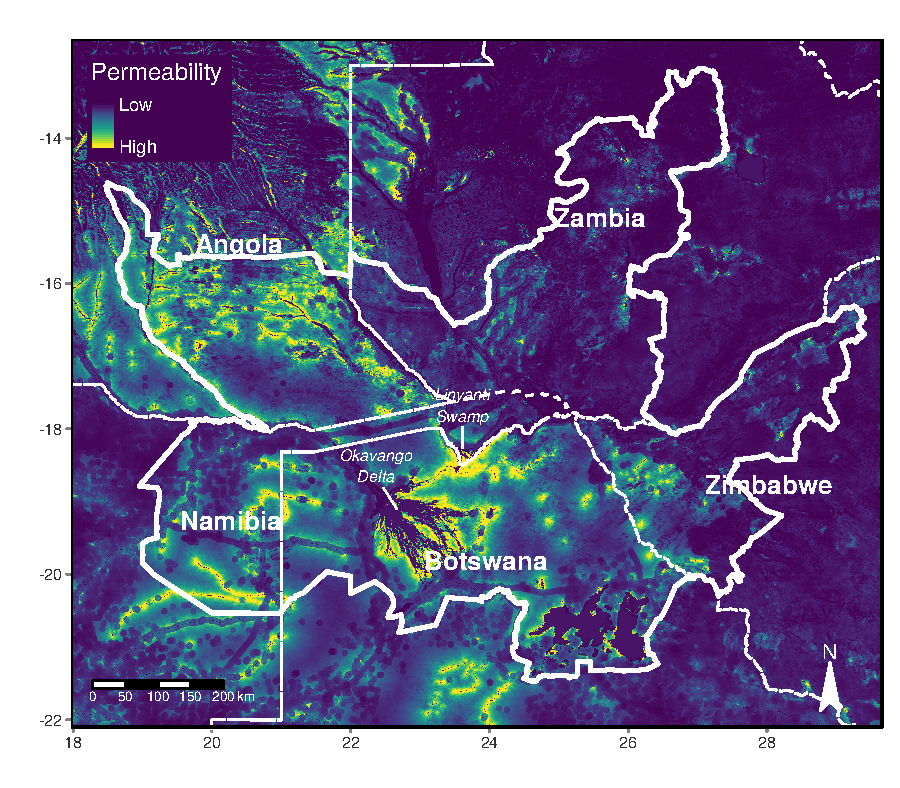
\includegraphics[width = \textwidth]{99_PermeabilityMap.pdf}
            \includegraphics[width = \textwidth]{99_PermeabilityMap2.pdf}
          \end{minipage}
        };
        \begin{scope}[x={(image.south east)},y={(image.north west)}]
           %  % next four lines will help you to locate the point needed by
           %  % forming a grid. comment these four lines in the final picture.↓
           % \draw[help lines,xstep=.1,ystep=.1] (0,0) grid (1,1);
           % \draw[help lines,xstep=.05,ystep=.05] (0,0) grid (1,1);
           % \foreach \x in {0,1,...,9} { \node [anchor=north] at (\x/10,0) {0.\x}; }
           % \foreach \y in {0,1,...,9} { \node [anchor=east] at (0,\y/10) {0.\y};}
           %  % upto here
            \draw[black, line width = 1pt] (0.389, 0.627) -- (0.080, 0.477);
            \draw[black, line width = 1pt] (0.582, 0.627) -- (0.980, 0.477);
            \draw[white, line width = 1pt] (0.675, 0.290) -- (0.720, 0.265);
            \draw[white, line width = 1pt] (0.840, 0.255) -- (0.800, 0.260);
            \draw[white, line width = 1pt] (0.807, 0.205) -- (0.752, 0.205);
        \end{scope}
    \end{tikzpicture}
    \caption{(a) Predicted permeability surface for the extent of the KAZA-TFCA.
    Permability was predicted by calculating selection scores \(w(x)\) for each
    pixel based on the pixel's underlying covariates. Areas that dispersers find
    easy to traverse are depicted in bright colors. Bold white lines delineate
    the borders of the KAZA-TFCA, whereas dashed white lines show country
    borders. (b) Detailed view of the Okavango Delta and Linyanti Swamp region,
    which appears to provide the most suitable landscape for dispersers. The
    white square highlights our core study area.}
    \label{PermeabilityMap}
  \end{center}
\end{figure}
\restoregeometry

\begin{table}[h]
  \caption{Comparison of median permeability across countries, separated
  according to areas within and outside the KAZA-TFCA, as well as within and
  outside protected areas. High values indicate high permeability, whereas low
  values correspond to low permeability.}
  \label{PermeabilityComp}
  \begin{center}
    \resizebox{0.65\textwidth}{!} {
      \begin{tabular}{llllllllr}
      & & \multicolumn{2}{c}{KAZA-TFCA} && \multicolumn{2}{c}{Protection Status} \\
      \cline{3-4} \cline{6-7}
      Country & & Inside & Outside & & Protected & Pastoral & & Overall \\
      \hline
      Angola & & 1.67 & 0.59 & & 1.67 & 0.60 & & 1.03 \\
      Namibia & & 0.91 & 0.49 & & 0.98 & 0.44 & & 0.59 \\
      Botswana & & 1.17 & 0.69 & & 1.37 & 0.62 & & 0.91 \\
      Zimbabwe & & 0.25 & 0.18 & & 0.32 & 0.17 & & 0.19 \\
      Zambia & & 0.26 & 0.12 & & 0.23 & 0.13 & & 0.15 \\
      \hline
      Overall & & 0.75 & 0.26 & & 0.74 & 0.27 & & 0.38 \\
      \end{tabular}
    }
  \end{center}
\end{table}

\subsection{Least-Cost Paths \& Least-Cost Corridors}
\Cref{LeastCost}a shows predicted LCPs and \Cref{LeastCost}b corresponding LCCs
for the extent of the KAZA-TFCA. Because LCPs identify the cheapest set of
pixels between two source points, they typically run along the center of LCCs
and traverse the same regions. The two figures thus essentially contain the same
information, albeit \Cref{LeastCost}b appears more detailed and reveals some
routes that would remain undetected in \Cref{LeastCost}a. Most notably, our
connectivity analysis revealed that several LCPs and LCCs traverse the
Chobe-Moremi region in northern Botswana (\Cref{LeastCost}a \circled{1}). In
fact, the highest frequented route in this region is passed by 637 LCPs, which
is reflected in a wide, dark red LCC in \Cref{LeastCost}b. Departing from this
central region, several high-frequency LCPs and LCCs emerge. One route
(\circled{2}) runs towards the north-western part of the KAZA-TFCA into the
Mavinga and Luengue-Luiana NPs. A further route (\circled{3}) meanders
north-east through unprotected area into the Kafue NP in Zambia. Another major
route (\circled{4}) extends east, into the Hwange NP in Zimbabwe and eventually
reaches the Matusadona NP (\circled{5}). A slightly less pronounced but still
distinguishable route (\circled{6}) originates from the Chobe-Moremi ecosystem
and runs south, through unprotected landscape, into the Central Kalahari NP in
Botswana. Alternatively, the corridor turns west (\circled{8}) and moves into
the Khaudum NP in Namibia (\circled{7}). Finally, another slightly less
accentuated path originates from southern Angola, moves through Botswana and
leads into the Khaudum NP in Namibia. Besides these medium- to high-frequency
routes, several low-frequency corridors exist and provide connectivity between
other protected areas. Strikingly, we found few direct LCPs and LCCs between
peripheral source points. That is, most paths and corridors connecting two
adjacent peripheral points detour through more central regions before they head
towards their destination at the periphery. As a consequence, there are several
peripheral regions providing little to no connectivity, as they are not crossed
by any LCPs or LCCs. Such regions are better visible in \Cref{LeastCost}b where
they appear as extended dark areas. Overall, there is a gradual decrease in the
density of LCPs and LCCs when moving from the central region towards the border
of the extended study area.

\newgeometry{left=30mm,right=30mm,top=0mm,bottom=20mm}
\begin{figure}[hbtp]
  \begin{center}
    \begin{tikzpicture}
        \node[anchor=south west,inner sep=0] (image) at (0,0,0) {
          \begin{minipage}{0.95\textwidth}
            \includegraphics[width = \textwidth]{99_LeastCostPaths.pdf}
            \includegraphics[width = \textwidth]{99_LeastCostCorrs.pdf}
          \end{minipage}
        };
        \begin{scope}[x={(image.south east)},y={(image.north west)}]
          % % next four lines will help you to locate the point needed by
          % % forming a grid. comment these four lines in the final picture.
          % \draw[help lines,xstep=.1,ystep=.1] (0,0) grid (1,1);
          % \draw[help lines,xstep=.05,ystep=.05] (0,0) grid (1,1);
          % \foreach \x in {0,1,...,9} {\node [anchor=north] at (\x/10,0) {0.\x};}
          % \foreach \y in {0,1,...,9} {\node [anchor=east] at (0,\y/10) {0.\y};}
          % % upto here
          \node[text=black, circle, scale=1, font=\bfseries, inner sep = 0.5pt
            , draw=black] (No1) at (0.400, 0.700){1};
          \node[text=black, circle, scale=1, font=\bfseries, inner sep = 0.5pt
            , draw=black] (No2) at (0.370, 0.760){2};
          \node[text=black, circle, scale=1, font=\bfseries, inner sep = 0.5pt
            , draw=black] (No3) at (0.585, 0.780){3};
          \node[text=black, circle, scale=1, font=\bfseries, inner sep = 0.5pt
            , draw=black] (No4) at (0.647, 0.697){4};
          \node[text=black, circle, scale=1, font=\bfseries, inner sep = 0.5pt
            , draw=black] (No5) at (0.910, 0.770){5};
          \node[text=black, circle, scale=1, font=\bfseries, inner sep = 0.5pt
            , draw=black] (No6) at (0.580, 0.658){6};
          \node[text=black, circle, scale=1, font=\bfseries, inner sep = 0.5pt
            , draw=black] (No7) at (0.410, 0.640){7};
          \node[text=black, circle, scale=1, font=\bfseries, inner sep = 0.5pt
            , draw=black] (No8) at (0.380, 0.665){8};
          \draw[black, line width = 1pt, densely dotted] (No1) -- (0.500, 0.710);
          \draw[black, line width = 1pt, densely dotted] (No2) -- (0.438, 0.760);
          \draw[black, line width = 1pt, densely dotted] (No3) -- (0.565, 0.805);
          \draw[black, line width = 1pt, densely dotted] (No4) -- (0.665, 0.685);
          \draw[black, line width = 1pt, densely dotted] (No5) -- (0.885, 0.765);
          \draw[black, line width = 1pt, densely dotted] (No6) -- (0.540, 0.650);
          \draw[black, line width = 1pt, densely dotted] (No7) -- (0.450, 0.645);
          \draw[black, line width = 1pt, densely dotted] (No8) -- (0.345, 0.690);
        \end{scope}
    \end{tikzpicture}
    \caption{(a) Source points (black dots) and corresponding least-cost paths
    leaving from protected areas (light grey). Note that only contiguous
    protected areas covering more than 700km\textsuperscript{2} are depicted.
    Circled numbers indicate some of the highest frequented least-cost paths
    that are mentioned in the main text. Continuous black lines indicate the
    borders of the KAZA-TFCA, whereas dashed black lines delineate
    country-borders. (b) Least-cost corridors between the same source points as
    illustrated in subfigure (a). For ease of spatial reference we also labeled
    national parks that are mentioned in the main text (dark-grey).}
    \label{LeastCost}
  \end{center}
\end{figure}
\restoregeometry

\newpage
\section{Discussion}
The goal of our study was to (1) assess landscape permeability for dispersing
wild dogs and to (2) subsequently use this knowledge to examine connectivity
across the greater extent of the KAZA-TFCA. To achieve these goals, we
parameterized a permeability model in which we used GPS data of 16 dispersing
wild dog coalitions to quantify their habitat preferences with respect to land
cover, protection status, and human influence. While we found significant
impacts of different land covers and human influence, the influence of
protection status was not statistically clear. We further applied the
parameterized permeability model and predicted a permeability surface for the
entire KAZA-TFCA, which depicted the ease at which dispersers crossed a specific
landscape. Finally, based on this permeability map, we computed LCPs and LCCs
between protectorates and thereby highlighted dispersal corridors of African
wild dogs.

\subsection{Permeability Model}
% Permeability Model: Land Cover, Water
Our most parsimonious permeability model revealed that, with respect to land
cover, dispersers strictly avoided areas covered by water (including swamps,
wetlands). This result corroborates previous research on wild dogs (e.g.
\cite{Abrahms.2017}) and is rather unsurprising, as the species is not well
adapted for moving through water. For residents, water is almost impermeable and
frequently serves as natural boundary to their home-ranges \citep{Cozzi.2013}.
It is conceivable that dispersers are more willing than residents to cross
waterbodies (\citeauthor{Cozzi.2019}, in review), but we did not include
residents in our analyses and could not test for such differences. Regardless of
that, water appears to pose a serious obstacle for dispersers and is therefore
likely to reduce landscape permeability for dispersing wild dogs.

% Permeability Model: Land Cover, DistanceToWater
While dispersers avoided moving \textit{through} water, they preferred moving
\textit{close to} water as indicated by avoidance of high distance to water.
While its effect was insignificant, inclusion of the covariate
\textit{DistanceToWater} strictly increased the AIC in all of our models and
suggests that distance to water influenced permeability negatively. We
hypothesize that high prey-availability (e.g. impala, kudu) in proximity to
water explains this result. It is well documented that water is a major driver
of wildlife and that it determines the distribution of many herbivores,
especially in dry biomes \citep{Western.1975}. For the Okavango Delta in
particular, it has been shown that prey abundance strongly correlates with the
extent of the flood \citep{Bonyongo.2005} and that an increasing concentration
of ungulates around remaining water-sources during the dry season might attract
dispersing wild dogs \citep{Ogutu.2014}. Following the same logic, however, apex
predators (e.g. lions, spotted hyenas) and resident wild dogs may also prefer
closeness to water \citep{Valeix.2009}, which may occasionally force dispersers
to move distant to water \citep{Ndaimani.2016} to avoid intraguild competition
\citep{Creel.1996, Mills.1997}. We could not control for the presence or absence
of apex predators or conspecifics because we lacked corresponding data, but
these considerations might explain why we did not find a statistically clear
effect of distance to water.

% Permeability Model: Land Cover, Trees & Shrubs
In line with existing literature on moving wild dogs \citep{Abrahms.2017}, we
found that dispersers avoided habitats with high percentages of tree cover,
whereas they preferred areas with high percentages of shrubs/grassland cover.
Comparable preferences were reported for residents, which typically reside in
savanna-like habitats but rarely inhabit areas with dense tree cover
\citep{Estes.2012}. This may be explained by wild dogs' hunting behavior, where
open habitats are favored because they offer increased visibility and thus
facilitate hunting \citep{Estes.1967}. Additionally, we found a strong negative
correlation between percentage cover by shrubs/grassland and percentage cover by
bareland (although we did not include bareland in our models). The observed
preference for shrubs/grassland could therefore also indicate an aversion to
bareland. Again, we hypothesize that this aversion is driven by low
prey-availability in non-vegetated habitats \citep{Pettorelli.2011}.
Unfortunately, we lacked detailed vegetation data and could not distinguish
vegetation types further.

% Permeability Model: Human Influence
Finally, considering human influence, we found that dispersers strongly avoided
human pressures arising from human density, farming, and roads. Previous
research on dispersing wild dogs was inconclusive about the impact of human
presence on permeability, as some researchers reported a high willingness of
dispersers to cross human-dominated landscapes \citep{DaviesMostert.2012},
whereas others found that humans are avoided almost entirely during dispersal
\citep{Masenga.2016}. Our results support the notion that dispersers strongly
avoid human-dominated areas, but we hypothesize that this finding depends on the
availability of alternative routes. The dipsersers monitored by
\cite{DaviesMostert.2012} originated from habitats almost exclusively surrounded
by humans, whereas our dipsersers departed from regions with various
possibilities to move through natural habitats. A lack of alternative routes
combined with strong inbreeding avoidance intrinsic in African wild dogs
\citep{McNutt.1996} might have forced the dispersers reported in
\cite{DaviesMostert.2012} to cross human-dominated landscapes despite a strong
aversion against humans. Although we found that our dispersers strictly avoided
humans, \citeauthor{Cozzi.2019} (in review) reports that human persecution
remains the main cause of mortality for dispersers, suggesting that avoidance is
not strong enough to prevent human-induced fatalities. We argue that human
influence remains a source of reduced landscape permeability and that the
proceeding transformation of natural landscapes into human altered habitats
continues to undermine wild dogs' ability to dipserse. Since our human influence
proxy did not include minor gravel roads, our finding that humans are avoided
does not contradict the observation that wild dogs preferably move on gravel
roads during activity \citep{Abrahms.2016}. With four-hourly GPS relocations we
felt that the temporal resolution was insufficient to depict such fine scale
effects \citep{Thurfjell.2014}.

\subsection{Permeability Surface}
% Permeability Surface
Our prediction of landscape permeability revealed vast regional differences.
Across the entire study area, northern Botswana stood out as it comprises the
highest density of highly permeable landscapes. The hospitality of this region
is caused by a combination of low human influence, low tree cover, high
shrubs/grassland cover and close distance to water. Thus, although swamps,
wetlands, and water (e.g. Okavango Delta, Linyanti Swamp) in northern Botswana
provide little permeability, their surroundings act as strong attractants to
dispersers. It is therefore not very surprising that the region serves as source
for the recolonization of surrounding habitats \citep{Cozzi.2013}. Moreover, we
found much higher permeability inside the KAZA-TFCA than outside its borders,
which suggests a good fit between the planned protectorates and areas that are
suitable for dispersal. We made similar observations for protection status,
where predicted permeabilities inside protectorates are much higher than in
pastoral regions. Yet, several highly permeable regions remain uncovered by the
KAZA-TFCA or other protected areas, proposing exciting opportunities for future
expansions of already existing protectorates. Across countries, we revealed that
Zambia and Zimbabwe offer the least permeable landscapes. Visual inspection of
our covariate-layers disclosed that this is mainly owed to severe anthropogenic
influence in Zambia and Zimbabwe. In contrast, Botswana and Angola host vast
uninhabited areas, resulting in more permeable landscapes for dispersers.
However, all of our predictions were based on observations from dispersing wild
dogs departing from northern Botswana, which might have introduced a bias in
estimated habitat preferences and resulting predictions.

\subsection{Least-Cost Paths \& Least-Cost Corridors}
% Least Cost Paths & Least Cost Corridors
Our LCP- and LCC-analyses disclosed several major movement corridors within the
extended study area and suggested a decent congruence between predicted
corridors and the layout of the KAZA-TFCA. That is, only few corridors run
outside the planned boundaries of the KAZA-TFCA and several currently
unprotected corridors will become protected with realization of the KAZA-TFCA.
For example, the high-frequency corridor running from southern Zambia into the
Kafue NP (\Cref{LeastCost}a \circled{3}) currently contains extended unprotected
sections that will be transformed into protectorates under the KAZA-TFCA. We
thus expect that dispersal between such regions will be vastly facilitated
thanks to the KAZA-TFCA. Our network of LCPs and LCCs furthermore highlighted
the Chobe-Moremi system in northern Botswana, which is traversed by several
LCPs and LCCs and seems to hold the potential to serve as central hub through
which dispersers gain access to more remote regions of the KAZA-TFCA. Still, our
predictions also indicated that movements between wild dog subpopulations may
often involve extended detours. This is especially the case for regions in the
northern sectors of the KAZA-TFCA. For instance, only few LCPs connect the
Zimbabwean and Zambian sectors, such that moving directly from the Matusadona NP
to the Kafue NP seems almost impossible and likely requires to make a detour
through the Chobe-Moremi region. Similarly, few LCPs directly link the Mavinga
NP in Angola and the Kafue NP in Zambia. Moreover, we discovered potential
dispersal routes between the Chobe-Moremi ecosystem and the Central Kalahari
NP that are not yet proclaimed protected areas. Nonetheless, a protected link
between the Central Kalahari NP and the Chobe-Moremi ecosystem might grant
southern populations invaluable access to the Chobe-Moremi-Hub and
subsequently to the entire KAZA-TFCA. In fact, \cite{Elliot.2014} identified a
similar corridor for dispersing lions, proposing that protecting the area would
benefit lions and wild dogs alike. The absence of direct LCPs and LCCs between
some regions of the KAZA-TFCA is likely owed to an impermeable landscape between
those regions and demonstrates that protection of such areas in their current
state would be futile. That is, impermeable landscapes first need to be
transformed into more permeable habitats before protection pays off. Although,
we noted that connectivity gradually decreases towards the borders of our study
area, this might partly be owed to boundary-effects \citep{Koen.2010}.
Interestingly, our network of LCPs and LCCs shows surprising similarities to
predicted movement corridors of dispersing lions \citep{Elliot.2014}.
Remarkably, corridors that we identified as high-frequency corridors are also
visible in the network presented by \cite{Elliot.2014}. This not only reinforces
confidence in our own predictions but it also suggests potential synergies
between conservation of the two species.

\subsection{Future Research}
% Future Research: Genetic Resistance
While we assessed landscape permeability purely based on GPS relocation
data, future studies could challenge and test our predictions using genetic data
\citep{Spear.2010}. Similar comparisons have been conducted for other species
and revealed a surprisingly high overlap between predicted landscape
permeability based on genetic and movement data \citep{Cushman.2010}. Genetic
data would also deepen our understanding of the degree to which subpopulations
admix and of the overall genetic diversity found in different subpopulations
\citep{Girman.2001}. Based on our connectivity network, we would expect to find
a low genetic diversity for populations that live in insufficiently connected
habitats, whereas populations residing at dispersal hotspots, such as the
Chobe-Linyanti ecosystem, should exhibit a relatively diverse gene-pool.

% Future Research: Better Covariates
Future research should also strive to improve representation of geo-referenced
covariates. Because we predicted connectivity for such an extensive area, we
were strongly limited in available and reliable land-cover data. As a result,
our representation of vegetation remained rather basic with only three
vegetation types (tree-cover, shrubs/grassland, bareland). Although there are a
few large-scale, high-resolution land cover datasets, such as Globeland's 30m
\citep{Chen.2015} and the European Space Agency's and 20m \citep{ESA.2019} land
cover datasets, we found their classifications often erroneous for our study
area. This is probably owed to the KAZA-TFCA's unique landscape and
corresponding difficulties in remote sensing satellite imagery using traditional
indices \citep{Wolski.2017}. Nevertheless, land cover is a very powerful
predictor of animal movement \citep{Thurfjell.2014}, which stresses the need for
more reliable land-cover data.

% Future Research: Competitor Presence
In a similar manner, we would desire better knowledge of the whereabouts of
other species. In particular, we would desire location data of apex predators,
potential prey, and conspecifics of wild dogs. It is well documented that
resident wild dogs frequently compete with other carnivores \citep{Creel.1998}
and we would expect to find competition between apex predators and dispersers
too. Furthermore, knowledge about the spatial distribution of prey could verify
our hypothesis that dispersers move along water due prey-availability. Lastly,
we could not control for the likelihood of encountering conspecifics during
dispersal . Yet, for dispersing meerkats, a species with surprisingly similar
social structure to wild dogs, it has been shown that the social landscape, i.e.
the presence or absence of conspecifics, strongly shapes behavior during
dispersal \citep{Cozzi.2018}. More specifically, it has been shown that
dispersers select for high density of conspecifics while still inside their
home-range, but that they avoid high densities of conspecifics once they leave
their natal home-range (we replicated this analysis for our core study area; see
\Cref{Appendix:SocialLandscape}). Spatially explicit knowledge about the
distribution of foreign wild dogs is thus desirable and would certainly deepen
our understanding of dispersal behavior. However, constructing meaningful and up
to date social landscapes is extremely challenging and requires vast amounts of
movement data, especially for such a wide-ranging species as the African wild
dog \citep{Pomilia.2015}.

% Global Resistance Mapping
Besides urging for more and better data, we also want to emphasize that our
analytical approach is neither limited to African wild dogs, nor to our study
area. All covariates used throughout this study are available on a global scale
and are likely to be important determinants of landscape permeability for other
species. Our framework could thus easily be used to assess connectivity for a
wide range of species, provided suitable relocation data of the species exists.
Expanding our analyses to other species would surely yield interesting insights
on the congruence of movement corridors of different species and thereby
highlight areas that are used by multiple species for dispersal.

% Simulating dispersal
To this end, we identified movement corridors between pre-defined start and
end-points. However, pre-defining end-points might not even be necessary, as one
could easily invert a parameterized iSSF and use it as a mechanistic movement
model to simulate dispersal. That is, one could define a set of source points at
locations where wild-dogs are assumed or known to reside and simulate dispersers
according to habitat-preferences that were derived using the iSSF framework.
End-points would not be restricted to a certain location and movement corridors
would emerge naturally as the result of a myriad of simulated dispersal events
(for an example of simulated dispersal events see
\Cref{Appendix:DispersalSimulation}).

\newpage
\subsection{Conclusion}
Our results demonstrate that indeed the majority of dispersal corridors are
covered by the planned protectorates of the KAZA-TFCA, suggesting that it will
severely contribute to the long-term viability of this species. Nevertheless,
several dispersal routes do exist outside the KAZA-TFCA and other protectorates
and suggest opportunities for further expansions in the future. Moreover, our
connectivity network of least-cost paths and least-cost corridors reveals
especially the Chobe-Linyanti region as central dispersal hub through which
dispersers gain access to more remote regions of the KAZA-TFCA. We therefore
stress the importance of northern Botswana for the conservation of this
charismatic species. Finally, our investigations showed that human pressure
remains a severe impediment to dispersal and strictly reduces landscape
connectivity. Successful conservation of the African wild dog is thus contingent
on the willingness of local authorities, policy makers, and land managers to
provide vast areas that are liberated from human strains. Ultimately, our work
contributes to the growing field of connectivity literature and has important
implications for the management and conservation of the endangered African wild
dog.

\newpage
\section{Acknowledgements}
All of this work would not have been possible without the aid of several helpful
people. I would first like to thank Prof. Arpat Ozgul, the leader and mastermind
of our research group, whose expertise in statistics, biological processes and
scientific writing was invaluable for my work. Moreover, I want to thank
Gabriele Cozzi for his excellent guidance, all the interesting discussions, his
constructive criticism, and of course his constant supply of freshly brewed
coffee. Particular gratitude goes to Dominik Behr who supervised my work on a
daily basis and greatly contributed to all aspects of the thesis. I genuinely
enjoyed the frequent meetings and brainstorms and I really feel privileged to
have had the opportunity of working with such a great scientist. I am also
greatly indebted to Prof. John Fieberg, who visited our department this summer
and invested a great amount of time to consult and improve all statistical
aspects of the thesis, as well as to deepen my personal understanding of
movement ecology. Furthermore, I thank the Okavango Research Institute, in
particular Piotr Wolski, for sharing all of their Python-scripts, floodmaps and
knowledge on developing dynamic floodmaps. Also, I want to thank Stefan Sommer
for sharing and teaching his hard earned knowledge on scientific writing.
Additionally, I want to thank all of my colleague master students who have been
wonderful companions and made the time at university a blast. Likewise, I thank
my parents for supporting all of my undertakings and for providing first class
shelter and food. Last, but most definitely not least, I also greatly thank my
girlfriend, who was always there for me and provided welcome distractions for my
mind.

\newpage
\begingroup
\singlespacing
\bibliography{Literatur}
\endgroup

\newpage
\appendix
\section{Appendix}
\subsection{Typical Flood Pulse}
\label{Appendix:FloodPulse}
\begin{figure}[h]
  \begin{center}
    \includegraphics[width = \textwidth]{99_FloodPulse.pdf}
    \caption{Sequence of figures showing a typical flood pulse throughout the
    year. The flood arrives from the north-western corner (so called
    ``pan-handle'') of the Okavango Delta and slowly descents through the delta
    in south-eastern direction, where it nourishes several tributaries. The
    extent of the flood peaks around August or September, after which it slowly
    retracts. Between December and March the reflectance properties of water and
    dryland change, which is why often no accurate floodmaps can be obtained for
    these months using remote sensing techniques.}
    \label{FloodPulse}
  \end{center}
\end{figure}

\newpage
\subsection{Reclassification of Protected Areas}
\label{Appendix:Reclassification}
\begin{table}[h]
  \caption{Reclassification of protected areas. Data on protection status was
  obtained from the \cite{PeaceParks.2019}. We simplified original categories to
  a binary classification of protected and unprotected (pastoral) areas. Any
  area that was not represented by one of the categories listed in
  \Cref{Reclassification} was deemed to be pastoral landscape.}
  \label{Reclassification}
  \begin{center}
    \resizebox{\textwidth}{!}{
      \begin{tabular}{llp{11cm}}
      \toprule
      \textbf{Original Category} &
        \textbf{Reclassification} &
          \textbf{Comment} \\
      \midrule
      Communal Conservancy &
        Protected &
          No comment\\
      Community Forest &
        Protected &
          No comment\\
      Conservancy &
        Protected &
          No comment\\
      Forest Reserve &
        Protected &
          No comment\\
      Game Management Area &
        Protected &
          No comment\\
      Game Park &
        Protected &
          No comment\\
      Game Ranch &
        Protected &
          No comment\\
      Game Reserve &
        Protected &
          No comment\\
      Hunting Reserve &
        Protected &
          No comment\\
      National Park &
        Protected &
          No comment\\
      National Park (not yet proclaimed) &
        \textit{Removed} &
          Since not yet proclaimed, we did not include this area as protected\\
      Overlap (GMA/FR) &
        Protected &
          Mixture between game management area and forest reserve\\
      Proposed &
        Protected &
          No comment\\
      Protected Area &
        Protected &
          No comment\\
      Recreation Park &
        \textit{Removed} &
          Marine reserve\\
      Safari Area &
        Protected &
          No comment\\
      Sanctuary &
        Protected &
          No comment\\
      State Forest &
        Protected &
          No comment\\
      Wildlife Management Area &
        Protected &
          No comment\\
      World Heritage Site &
        Protected &
          No comment\\
      Freehold Conservancy &
        Protected &
          No comment\\
      \bottomrule
      \end{tabular}
    }
  \end{center}
\end{table}

\newpage
\subsection{Road Categories}
\label{Appendix:RoadCategories}
\begin{table}[h]
  \caption{Description of road types, as sourced from Open Street Map's mapping
  guide (\url{https://wiki.openstreetmap.org/wiki/Key:highway}). Roads types
  that were considered for the purpose of this study are shaded in light gray.}
  \label{RoadsDescription}
  \begin{center}
    \resizebox{\textwidth}{!}{
      \begin{tabular}{llp{13cm}}
      \toprule
      \textbf{Group} &
        \textbf{Subgroup} &
          \textbf{Description} \\
      \midrule
      \rowcolor[gray]{0.80}
      Roads &
        motorway &
          A restricted access major divided highway, normally with 2 or more
          running lanes plus emergency hard shoulder. Equivalent to the
          Freeway, Autobahn, etc. \\
      \rowcolor[gray]{0.80}
      Roads &
        trunk &
          The most important roads in a country's system that aren't
          motorways. Need not necessarily be a divided highway. \\
      \rowcolor[gray]{0.80}
      Roads &
        primary &
          The next most important roads in a country's system. Often link
          larger towns. \\
      \rowcolor[gray]{0.80}
      Roads &
        secondary &
          The next most important roads in a country's system. Often link
          towns. \\
      Roads &
        tertiary &
          The next most important roads in a country's system. Often link
          smaller towns and villages \\
      Roads &
        unclassified &
          The least important thorough roads in a country's system, i.e. minor
          roads of a lower classification than tertiary, but which serve a
          purpose other than access to properties. Often link villages and
          hamlets. \\
      Roads &
        residential &
          Roads which serve as an access to housing, without function of
          connecting settlements. Often lined with housing. \\
      Roads &
        service &
          For access roads to, or within an industrial estate, camp site,
          business park, car park etc. \\
      \rowcolor[gray]{0.80}
      Link roads &
        motorway\_link &
          The link roads (sliproads/ramps) leading to/from a motorway from/to
          a motorway or lower class highway. Normally with the same motorway
          restrictions. \\
      \rowcolor[gray]{0.80}
      Link roads &
        trunk\_link &
          The link roads (sliproads/ramps) leading to/from a trunk road
          from/to a trunk road or lower class highway. \\
      \rowcolor[gray]{0.80}
      Link roads &
        primary\_link &
          The link roads (sliproads/ramps) leading to/from a primary road
          from/to a primary road or lower class highway. \\
      \rowcolor[gray]{0.80}
      Link roads &
        secondary\_link &
          The link roads (sliproads/ramps) leading to/from a secondary road
          from/to a secondary road or lower class highway. \\
      Link roads &
        tertiary\_link &
          The link roads (sliproads/ramps) leading to/from a tertiary road
          from/to a tertiary road or lower class highway. \\
      Special road types &
        living\_street &
          For living streets, which are residential streets where pedestrians
          have legal priority over cars, speeds are kept very low and where
          children are allowed to play on the street. \\
      Special road types &
        pedestrian &
          For roads used mainly/exclusively for pedestrians in shopping and
          some residential areas which may allow access by motorised vehicles
          only for very limited periods of the day. \\
      Special road types &
        track &
          Roads for mostly agricultural or forestry uses. \\
      Special road types &
        bus\_guideway &
          A busway where the vehicle is guided by the way (though not a railway)
          and is not suitable for other traffic. \\
      Special road types &
        escape &
          For runaway truck ramps, runaway truck lanes, emergency escape
          ramps, or truck arrester beds. It enables vehicles with braking
          failure to safely stop. \\
      Special road types &
        raceway &
          A course or track for racing \\
      Special road types &
        road &
          A road/way/street/motorway/etc. of unknown type. It can stand for
          anything ranging from a footpath to a motorway. \\
      \bottomrule
      \end{tabular}
    }
  \end{center}
\end{table}

\newpage
\subsection{Covariate Sources}
\label{Appendix:Sources}
\begin{table}[h]
  \begin{center}
    \caption{Sources from which we obtained our set of geo-referenced
    covariates, as well as an indicator of their original resolution and the
    method used for adjusting the resolution to 250m x 250m.}
    \label{Sources}
    \resizebox{\textwidth}{!} {
      \begin{tabular}{llp{4cm}p{4cm}p{7cm}}
      \hline
      \textbf{Category} &
        \textbf{Covariate} &
          \textbf{Resolution} &
            \textbf{Resampling} &
              \textbf{Source(s)} \\
      \midrule
      Land Cover
        & Water
          & 30m x 30m (static), 500m x 500m (dynamic)
            & Mode of each 250x x 250m cell (static), disaggregation to 250m x 250m (dynamic)
              & \cite{Chen.2015}, \cite{Schaaf.2015}, \cite{Yamazaki.2019} \\
      Land Cover
        & Dryland
          & 30m x 30m (static), 500m x 500m (dynamic)
            & Mode of each 250x x 250m cell (static), disaggregation to 250m x 250m (dynamic)
              & \cite{Chen.2015}, \cite{Schaaf.2015}, \cite{Yamazaki.2019} \\
      Land Cover
        & DistanceToWater
          & 30m x 30m (static), 500m x 500m (dynamic)
            & Mode of each 250x x 250m cell (static), disaggregation to 250m x 250m (dynamic)
              & \cite{Chen.2015}, \cite{Schaaf.2015}, \cite{Yamazaki.2019} \\
      Land Cover
        & Shrubs/Grassland
          & 250m x 250m
            & NA
              & \cite{Dimiceli.2015} \\
      Land Cover
        & Trees
          & 250m x 250m
            & NA
              & \cite{Dimiceli.2015} \\
      Land Cover
        & Bareland
          & 250m x 250m
            & NA
              & \cite{Dimiceli.2015} \\
      \hdashline
      Protection Status
        & Protected
          & NA
            & NA
              & \cite{PeaceParks.2019} \\
      Protection Status
        & Pastoral
          & NA
            & NA
              & \cite{PeaceParks.2019} \\
      \hdashline
      Human Influence
        & HumansBuffer5000
          & 30m x 30m
            & Sum of each 250m x 250m cell
              & \cite{Facebook.2019}, \cite{OpenStreetMap.2019}, \cite{Chen.2015}, \cite{Xiong.2017}\\
      Human Influence
        & DistanceToRoads
          & NA
            & NA
              & \cite{Facebook.2019}, \cite{OpenStreetMap.2019}, \cite{Chen.2015}, \cite{Xiong.2017}\\
      Human Influence
        & RoadCrossing
          & NA
            & NA
              & \cite{Facebook.2019}, \cite{OpenStreetMap.2019}, \cite{Chen.2015}, \cite{Xiong.2017}\\
      \hline
      \end{tabular}
    }
  \end{center}
\end{table}


\newpage
\subsection{Model Selection Results}
\label{AICs}
\begin{table}[h]
  \caption{Results from the forward model selection procedure based on AIC
  \citep{Burnham.2002} for our permeability model. Weights were calculated
  using: \(\text{AIC-Weight}_i = \frac{e^{-0.5} \Delta \text{AIC}_i} {\sum_{i =
  1}^n e^{-0.5} \Delta \text{AIC}_i} \). The most parsimonious model (shaded in
  light gray) outperformed all other models (\(\Delta AIC > \) 2) and received a
  weight of one. The model in the last row did not converge and no AIC value
  could be obtained. (*) represents the fixed covariates \(cos(ta\_)\) and
  \(log(sl\_)\).}
  \label{ModelAICs}
  \begin{center}
    \resizebox{\textwidth}{!}{
      \begin{tabular}{lllll}
      \toprule
      \textbf{Covariates} &
        \textbf{AIC} &
          \textbf{\(\Delta\)AIC} &
            \textbf{AIC-Weight} &
              \textbf{LogLik} \\
      \midrule
      \rowcolor[gray]{0.80}
      (*), Water, DistanceToWater, Shrubs/Grassland, HumansBuff5000, Trees &
        89841.85 &
          0.00 &
            1.00 &
              -44905.93 \\
      (*), Water, DistanceToWater, Shrubs/Grassland, HumansBuff5000, Trees, DistanceToRoads &
        89844.46 &
          2.61 &
            0.00 &
              -44905.23 \\
      (*), Water, DistanceToWater, Shrubs/Grassland, HumansBuff5000, Trees, Protected &
        89845.78 &
          3.93 &
            0.00 &
              -44905.89 \\
      (*), Water, DistanceToWater, Shrubs/Grassland, HumansBuff5000 &
        89847.96 &
          6.11 &
            0.00 &
              -44910.98 \\
      (*), Water, DistanceToWater, Shrubs/Grassland, HumansBuff5000, Trees,
      RoadCrossing &
        89848.24 &
          6.38 &
            0.00 &
              -44905.12 \\
      (*), Water, DistanceToWater, Shrubs/Grassland, HumansBuff5000, Trees,
      DistanceToRoads, Protected &
        89848.45 &
          6.60 &
            0.00 &
              -44905.22 \\
      (*), Water, DistanceToWater, Shrubs/Grassland, Trees
        & 89850.51 &
          8.66 &
            0.00 &
              -44912.26 \\
      (*), Water, DistanceToWater, Shrubs/Grassland, HumansBuff5000,
      DistanceToRoads &
        89850.81 &
          8.96 &
            0.00 &
              -44910.40 \\
      (*), Water, DistanceToWater, Shrubs/Grassland, HumansBuff5000, Trees, DistanceToRoads, RoadCrossing &
        89850.87 &
          9.02 &
            0.00 &
              -44904.44 \\
      (*), Water, DistanceToWater, Shrubs/Grassland, HumansBuff5000, Protected &
        89851.91 &
          10.06 &
            0.00 &
              -44910.96 \\
      (*), Water, DistanceToWater, Shrubs/Grassland, HumansBuff5000, RoadCrossing &
        89854.42 &
          12.57 &
            0.00 &
              -44910.21 \\
      (*), Water, DistanceToWater, Shrubs/Grassland &
        89856.89 &
          15.03 &
            0.00 &
              -44917.44 \\
      (*), Water, DistanceToWater, Shrubs/Grassland, DistanceToRoads &
        89858.78 &
          16.92 &
            0.00 &
              -44916.39 \\
      (*), Water, DistanceToWater, Shrubs/Grassland, Protected &
        89860.44 &
          18.59 &
            0.00 &
              -44917.22 \\
      (*), Water, DistanceToWater, Shrubs/Grassland, RoadCrossing &
        89862.66 &
          20.81 &
            0.00 &
              -44916.33 \\
      (*), Water, DistanceToWater, HumansBuff5000 &
        89870.14 &
          28.29 &
            0.00 &
              -44924.07 \\
      (*), Water, DistanceToWater &
        89877.72 &
          35.87 &
            0.00 &
              -44929.86 \\
      (*), Water, DistanceToWater, DistanceToRoads &
        89880.07 &
          38.22 &
            0.00 &
              -44929.04 \\
      (*), Water, DistanceToWater, Protected &
        89881.39 &
          39.54 &
            0.00 &
              -44929.70 \\
      (*), Water, DistanceToWater, Trees &
        89881.57 &
          39.72 &
            0.00 &
              -44929.79 \\
      (*), Water, DistanceToWater, RoadCrossing &
        89883.48 &
          41.63 &
            0.00 &
              -44928.74 \\
      (*), Water, HumansBuff5000 &
        89887.27 &
          45.42 &
            0.00 &
              -44934.64 \\
      (*), Water &
        89894.64 &
          52.79 &
            0.00 &
              -44940.32 \\
      (*), Water, DistanceToRoads &
        89897.24 &
          55.39 &
            0.00 &
              -44939.62 \\
      (*), Water, Protected &
        89898.47 &
          56.62 &
            0.00 &
              -44940.24 \\
      (*), Water, Trees &
        89898.53 &
          56.67 &
            0.00 &
              -44940.26 \\
      (*), Water, RoadCrossing &
        89900.73 &
          58.88 &
            0.00 &
              -44939.37 \\
      (*), Shrubs/Grassland &
        89999.47 &
          157.62 &
            0.00 &
              -44992.73 \\
      (*), DistanceToWater &
        90001.72 &
          159.87 &
            0.00 &
              -44993.86 \\
      (*), HumansBuff5000 &
        90056.07 &
          214.22 &
            0.00 &
              -45021.04 \\
      (*), Trees &
        90059.55 &
          217.69 &
            0.00 &
              -45022.77 \\
      (*), DistanceToRoads &
        90067.62 &
          225.76 &
            0.00 &
              -45026.81 \\
      (*), Protected &
        90067.85 &
          226.00 &
            0.00 &
              -45026.93 \\
      (*), RoadCrossing &
        90069.86 &
          228.00 &
            0.00 &
              -45025.93 \\
      (*), Water, Shrubs/Grassland &
        \(NA\) &
          \(NA\) &
            0.00 &
              \(NA\) \\
      \bottomrule
      \end{tabular}
    }
  \end{center}
\end{table}

\newpage
\subsection{Further Investigations}
We have been working on further investigations that did not fit the main text
and were thus moved to the Appendix of this thesis. \Cref{SchematicOverview}
gives an overview of how these additional investigations integrate into our main
work. Our main work is described in the blue boxes, which resulted in the
identification of LCPs and LCCs. However, as we have emphasized in the
discussion, the applicability of the iSSF framework expands beyond the
estimation of movement and habitat preferences and it could, in fact, be used to
simulate animal movement. We thus engaged in fitting a movement model that was
specifically intended to simulate dispersal events (red boxes). Using this
model, we simulated 1000 dispersal events across the surroundings of our core
study area and qualitatively assessed the outcome. Corresponding methods and
results are reported in \Cref{Appendix:DispersalSimulation}. Furthermore, we
motivated that data on the social landscape of dispersers would deepen our
understanding of how dispersers are influenced by the presence or absence of
conspecifics, apex predators, and prey. Although we lacked proper GPS relocation
data of apex predators and prey, we collected a considerable amount of movement
data from resident wild dogs residing in our core study area. These data cover
the periods of almost all of our dispersal events and thus hold the potential
for modeling a social landscape for our dispersers. Hence, we modeled such a
landscape for the extent of our core study area and used it as additional
covariate to parameterize a social model (yellow box). Corresponding methods and
results are reported in \Cref{Appendix:SocialLandscape}.

\begin{figure}[h]
  \begin{center}
    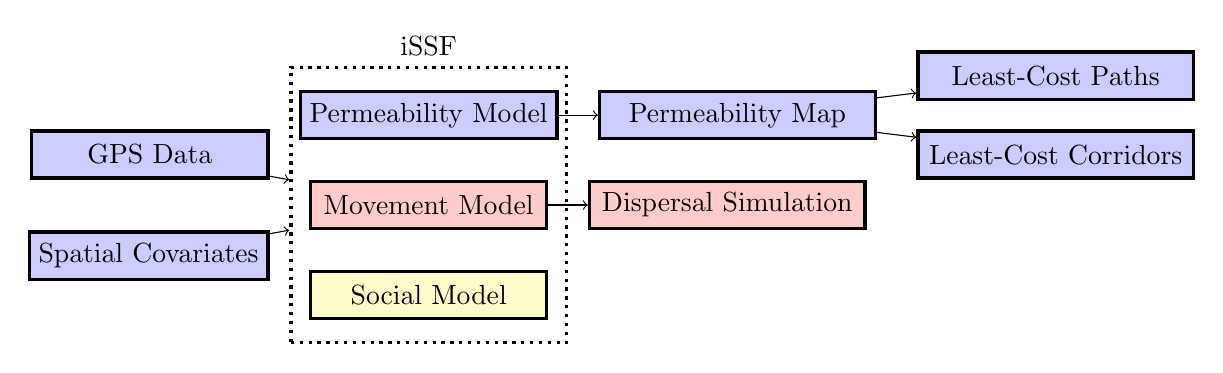
\begin{tikzpicture}[node distance=5mm and 5mm]
      \node (mod2) [nonterminal
        , minimum width = 30mm
        , fill          = red!20
        ] {Movement Model};
      \node (mod1) [nonterminal
        , above         = of mod2
        , fill          = blue!20
        , minimum width = 30mm
        ] {Permeability Model};
      \node (mod3) [nonterminal
        , below         = of mod2
        , fill          = yellow!20
        , minimum width = 30mm
        ] {Social Model};
      \node (dat1) [nonterminal
        , above left    = of mod2
        , fill          = blue!20
        , yshift        = -5mm
        , minimum width = 30mm
        ] {GPS Data};
      \node (dat2) [nonterminal
        , below left    = of mod2
        , fill          = blue!20
        , yshift        = +5mm
        , minimum width = 30mm
        ] {Spatial Covariates};
      \node (for1) [nonterminal
        , right         = of mod1
        , fill          = blue!20
        , minimum width = 35mm
        ] {Permeability Map};
      \node (forfor1) [nonterminal
        , right         = of for1
        , fill          = blue!20
        , minimum width = 35mm
        , yshift        = +5mm
        ] {Least-Cost Paths};
      \node (forfor2) [nonterminal
        , right         = of for1
        , fill          = blue!20
        , minimum width = 35mm
        , yshift        = -5mm
        ] {Least-Cost Corridors};
      \node (for2) [nonterminal
        , right         = of mod2
        , fill          = red!20
        , minimum width = 35mm
        ] {Dispersal Simulation};
      \node (box) [draw
        , dotted
        , very thick
        , minimum width   = 35mm
        , minimum height  = 35mm
        ] {};
      \node [above = of box, yshift = -5mm] {iSSF};
      \path (dat1) edge[->] (box);
      \path (dat2) edge[->] (box);
      \path (mod1) edge[->] (for1);
      \path (mod2) edge[->] (for2);
      \path (for1) edge[->] (forfor1);
      \path (for1) edge[->] (forfor2);
    \end{tikzpicture}
    \caption{Schematic overview of our methodological approaches. The blue boxes
    highlight our main line of work which resulted in the identification of
    least-cost paths and least-cost corridors. The red boxes show how we
    additionally used the iSSF framework to specifically analyze movement
    behavior and subsequently to simulate dispersal events. Finally, the yellow
    box indicates our attempt to use the iSSF framework to model and analyze the
    influence of the social landscape on dispersal behavior.}
    \label{SchematicOverview}
  \end{center}
\end{figure}

\newpage
\subsection{Movement Model \& Dispersal Simulation}
\label{Appendix:DispersalSimulation}
\subsubsection{Methods}
To gain more detailed insights into the movement behavior of dispersing wild
dogs and to simulate dispersal events, we fitted a more complex movement model.
The movement model still contained the most parsimonious permeability model, but
in addition included interaction terms between movement metrics (i.e.
\(cos(ta\_)\), \(log(sl\_\))) and environmental covariates (e.g. water). For
instance, for the environmental covariate \textit{Water}, we created the
interaction terms \textit{cos(ta\_):Water} and \textit{log(sl\_):Water}. These
interactions served to learn how dispersers moved differently, depending on
environmental covariates (for comparable work see \cite{Prokopenko.2017}). We
applied the same modeling framework as explained in \Cref{Modeling} and ran
forward model selection based on AIC to identify the most parsimonious movement
model. That is, we departed from the permeability model and iteratively added
interactions with movement metrics. Note that we applied forward model selection
only on the newly identified interactions, but not for the terms that were
already in the permeability model. Since we attempted to keep our simulation
simple, we did not average models with positive AIC-weights but simply
identified the most parsimonious movement model.

Using the most parsimonious movement model, we simulated 1000 dispersal events
departing from our core study area. The simulation basically resembled an
inverted iSSF function and was set up as follows. First, we sampled a random
starting location within our core study area. Second, we assigned a random
orientation in order to be able to calculate turning angles. Third, we created
an array of 25 random steps (i.e. one stratum) following the same procedure as
described in \Cref{Modeling}. Fourth, we extracted environmental covariates
along each of the generated random steps and calculated the metrics listed in
\Cref{ExtractedCovars}. Fifth, we applied \Cref{EQ2} using parameter estimates
from the movement model and calculated the selection score \(w(x)\) of each of
the 25 random steps. Sixth, we identified and realized the step with the highest
selection score and determined the new location. We then repeated steps three to
six until 200 steps were realized. To deal with dispersers that approached a map
boundary, our simulation included the options to either stop the simulation and
skip to the next disperser, or to remove any random step ranging outside the
study area, thereby forcing the simulated disperser to stay within the
boundaries. None of the simulated dispersers approached a map boundary within
200 steps and the decision did not influence our findings. Although we ran the
simulation only for dispersers departing from our core study area, one could
easily expand the simulation to include multiple sources and thereby check how
well these sources are connected.

\newpage
\subsubsection{Results}
Along with the original covariates contained in the permeability model, our most
parsimonious movement model (see \Cref{ModelAICs2} and
\Cref{MovementModelResults}) retained three additional interactions (see red box
in \Cref{MovementModel}a). Since the sign and direction of the effects contained
in the permeability model did not markedly change, we only report on the newly
added interactions between environmental covariates and movement metrics. For an
easier interpretation of how these interactions influenced habitat selection and
movement patterns during dispersal, we prepared surface plots as depicted in
\Cref{MovementModel}b. These surface plots revealed that dispersers preferred
long steps (i.e. a high movement rate) when water cover was low, whereas they
preferred short steps (i.e. a low movement rate) when water cover was high (see
\Cref{MovementModel}b1). Furthermore, dispersers were indifferent between high
and low turning angles in proximity to water, but clearly preferred low turning
angles (i.e. a high \(cos(ta\_)\)) when distance to water was high (see
\Cref{MovementModel}b2). Finally, dispersers preferably realized steps with low
turning angles when human influence was low, whereas they preferably realized
low turning angles when human influence was high (see \Cref{MovementModel}b3).

\begin{figure}[hbtp]
  \begin{center}
    \begin{tikzpicture}
        \node[anchor=south west,inner sep=0] (image) at (0,0,0) {
          \begin{minipage}{0.95\textwidth}
            \begin{center}
              \includegraphics[width = 0.80\textwidth]
                {99_MovementModel.pdf}\\
              \includegraphics[width = 1\textwidth]
                {99_MovementModel(Interactions).pdf}
            \end{center}
          \end{minipage}
        };
        \begin{scope}[x={(image.south east)},y={(image.north west)}]
           %  % next four lines will help you to locate the point needed by
           %  % forming a grid. comment these four lines in the final picture.↓
           % \draw[help lines,xstep=.1,ystep=.1] (0,0) grid (1,1);
           % \draw[help lines,xstep=.05,ystep=.05] (0,0) grid (1,1);
           % \foreach \x in {0,1,...,9} { \node [anchor=north] at (\x/10,0) {0.\x}; }
           % \foreach \y in {0,1,...,9} { \node [anchor=east] at (0,\y/10) {0.\y};}
           %  % upto here
            \draw [red, dashed] (0.13, 0.50) rectangle (0.405, 0.645);
        \end{scope}
    \end{tikzpicture}
    \caption{(a) Results from the most parsimonious movement model. Negative
    coefficients indicate avoidance of a covariate, positive coefficients
    selection of a covariate. Whiskers delineate the 95\%-CIs for estimated
    parameters. The intercept is meaningless in the iSSF framework and was thus
    omitted. (b) Corresponding surface plots for two-way interactions. Light
    areas depict a combination of covariates that were preferred by dispersers,
    whereas darker areas correspond to avoided combinations. The absolute values
    along the axes have no meaning as they were normalized to 0 (low) and 1
    (high).}
    \label{MovementModel}
  \end{center}
\end{figure}

\newpage
\noindent \Cref{Simulations}a shows the outcome of the dispersal simulations.
For better visibility of high-frequency routes, we rasterized all simulated
trajectories and computed a heatmap depicting areas that were crossed by many
simulated trajectories. Unsurprisingly, we found that the dispersal trajectories
clearly reflected preferences that we identified earlier. For instance, most
trajectories were quite directional, avoided crossing a waterbody, ran along
waterbodies and avoided human-dominated areas. More interestingly, however, the
resulting heatmap closely resembled our permeability surface (see
\Cref{Simulations}b). That is, areas providing high permeability were typically
crossed by more simulated trajectories. Yet, the heatmap also showed that some
regions are almost impossible to reach, even if they provide highly permeable
landscapes. For example, although the western section of the Okavango Delta
holds highly permeable landscapes, no simulated trajectory reached these areas.
In contrast, many trajectories ventured towards east, some of them even crossing
the border to Zimbabwe. The reason that no trajectory reached the eastern part
of the Delta is likely owed to severe human influence and an impermeable flood
that together posed an insurmountable barrier and prevented dispersers from
traversing the landscape.

\begin{figure}[h]
  \begin{center}
    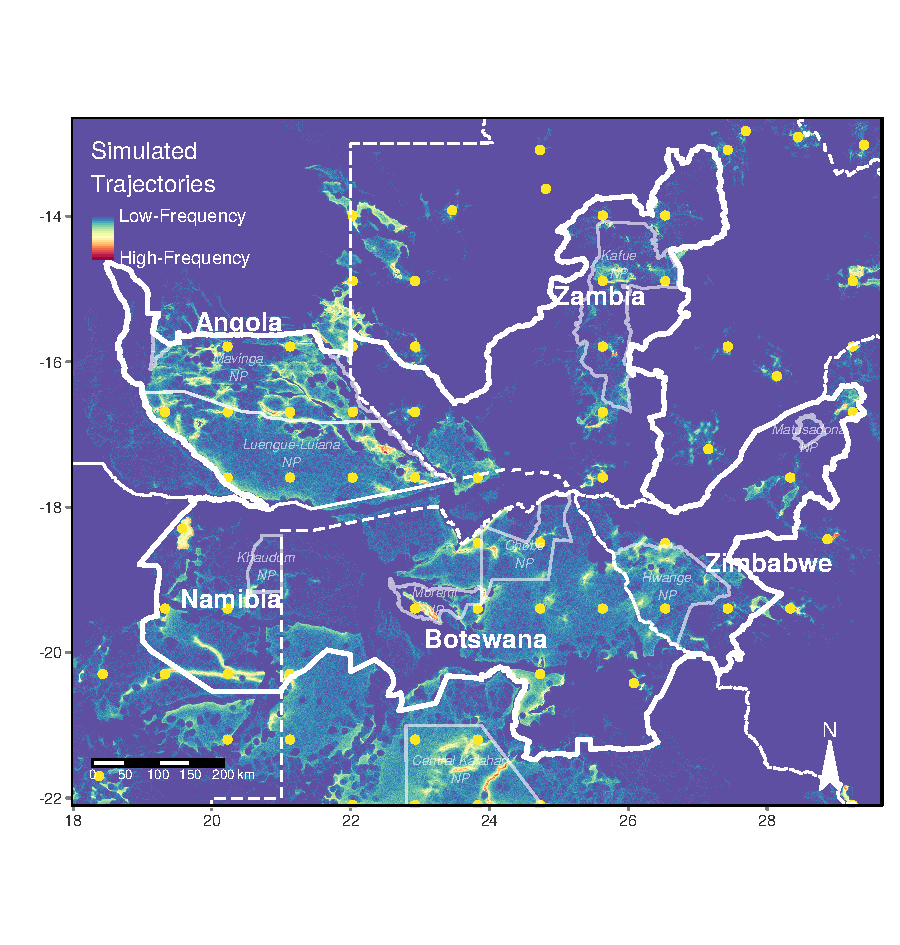
\includegraphics[width = 0.83\textwidth]{99_Simulations.pdf}
    \caption{(a) Heatmap of 1000 simulated dispersal events departing from the
    core study area (white square) in northern Botswana (countries with dashed
    white lines). (b) Permeability map for the same extent, showing that
    simulated dispersal trajectories typically cover highly permeable
    landscapes.}
    \label{Simulations}
  \end{center}
\end{figure}

\newpage
\begin{table}[h]
  \caption{Results from the forward model selection procedure based on AIC
  \citep{Burnham.2002} for our movement model. Weights were calculated using:
  \(\text{AIC-Weight}_i = \frac{e^{-0.5} \Delta \text{AIC}_i} {\sum_{i = 1}^n
  e^{-0.5} \Delta \text{AIC}_i} \). (*) represents all covariates from the most
  parsimonious permeability model, i.e. \(cos(ta\_)\), \(log(sl\_\)),
  \textit{Water}, \textit{DistanceToWater}, \textit{Shrubs/Grassland},
  \textit{HumansBuff5000}, and \textit{Trees}. To keep the table short we only
  included models with positive AIC weights. We abstained from averaging models
  with AIC-weight \(>\) 0 because we attempted to keep our simulation simple.}
  \label{ModelAICs2}
  \begin{center}
    \resizebox{\textwidth}{!}{
      \begin{tabular}{llllll}
      \toprule
      \textbf{Covariates} &
        \textbf{AIC} &
          \textbf{\(\Delta\)AIC} &
            \textbf{AIC-Weight} &
              \textbf{LogLik} \\
      \midrule
      \rowcolor[gray]{0.80}
        (*),
        log(sl\_):Water, cos(ta\_):DistanceToWater, cos(ta\_):HumansBuff5000 &
          89814.19 &
            0.00 &
              0.13 &
                -44889.10 \\
        (*), log(sl\_):Water, cos(ta\_):DistanceToWater, cos(ta\_):Trees &
          89814.37 &
            0.17 & 0.12 &
              -44889.18 \\
        (*), log(sl\_):Water, cos(ta\_):DistanceToWater &
          89814.46 &
            0.27 &
              0.11 &
                -44890.23 \\
        (*), log(sl\_):Water, cos(ta\_):DistanceToWater, cos(ta\_):HumansBuff5000, cos(ta\_):Trees &
          89814.87 &
            0.68 &
              0.09 &
                -44888.44 \\
        (*), log(sl\_):Water, cos(ta\_):DistanceToWater, cos(ta\_):HumansBuff5000, cos(ta\_):Shrubs &
          89815.32 &
            1.13 &
              0.07 &
                -44888.66 \\
        (*), log(sl\_):Water, cos(ta\_):DistanceToWater, cos(ta\_):Shrubs &
          89815.34 &
            1.15 &
              0.07 &
                -44889.67 \\
        (*), log(sl\_):Water, cos(ta\_):DistanceToWater, cos(ta\_):HumansBuff5000, log(sl\_):Shrubs &
          89815.40 &
            1.20 &
              0.07 &
                -44888.70 \\
        (*), log(sl\_):Water, cos(ta\_):DistanceToWater, log(sl\_):Shrubs &
          89815.67 &
            1.48 &
              0.06 &
                -44889.84 \\
        (*), log(sl\_):Water, cos(ta\_):DistanceToWater, cos(ta\_):HumansBuff5000, log(sl\_):HumansBuff5000 &
          89815.94 &
            1.75 &
              0.05 &
                -44888.97 \\
        (*), log(sl\_):Water, cos(ta\_):DistanceToWater, cos(ta\_):HumansBuff5000, cos(ta\_):Trees, log(sl\_):Shrubs &
          89816.08 &
            1.89 &
              0.05 &
                -44888.04 \\
        (*), log(sl\_):Water, cos(ta\_):DistanceToWater, cos(ta\_):HumansBuff5000, log(sl\_):DistanceToWater &
          89816.14 &
            1.95 &
              0.05 &
                -44889.07 \\
        (*), log(sl\_):Water, cos(ta\_):DistanceToWater, cos(ta\_):HumansBuff5000, cos(ta\_):Water &
          89816.16 &
            1.97 &
              0.05 &
                -44889.08 \\
        (*), log(sl\_):Water, cos(ta\_):DistanceToWater, log(sl\_):HumansBuff5000 &
          89816.18 &
            1.99 &
              0.05 &
                -44890.09 \\
        (*), log(sl\_):Water, cos(ta\_):DistanceToWater, cos(ta\_):HumansBuff5000, log(sl\_):Trees &
          89816.19 &
            2.00 &
              0.05 &
                -44889.10 \\
      \bottomrule
      \end{tabular}
    }
  \end{center}
\end{table}

\begin{table}[h]
  \caption{Selection coefficients as derived from the most parsimonious movement
  model. The movement model was a modified permeability model to which we added
  additional interaction terms between movement metrics and environmental
  covariates (e.g. \(Water:cost(ta\_)\)) in order to learn about how movement
  behavior changes depending on the environmental covariates.}
  \label{MovementModelResults}
  \begin{center}
    \resizebox{0.5\textwidth}{!}{
      \begin{tabular}{llllll}
      \toprule
      Covariate & Coefficient & SE & p-value \\
      \midrule
      cos(ta\_) & 0.149 & 0.045 & 0.001 \\
      log(sl\_) & 0.053 & 0.019 & 0.005 \\
      Water & -0.265 & 0.090 & 0.003 \\
      DistanceToWater & -0.272 & 0.226 & 0.230 \\
      Shrubs & 0.391 & 0.082 & 0.000 \\
      HumansBuff5000 & -0.466 & 0.203 & 0.022 \\
      Trees & -0.177 & 0.072 & 0.013 \\
      log(sl\_):Water & -0.040 & 0.008 & 0.000 \\
      cos(ta\_):DistanceToWater & 0.115 & 0.038 & 0.003 \\
      cos(ta\_):HumansBuff5000 & -0.047 & 0.031 & 0.134 \\
       \bottomrule
      \end{tabular}
    }
  \end{center}
\end{table}

\newpage
\subsection{Social Model}
\label{Appendix:SocialLandscape}
\subsubsection{Methods}
We used GPS relocation data of resident wild dogs and calculated a
geo-referenced stack of layers to which we refer as the \textit{social
landscape}. The social landscape was a collection of raster-layers, each
depicting the probability of encountering a resident group in a given pixel and
month. The social landscape was updated every month, using a moving window that
took into account six months of relocation data. For instance, the social
landscape dated July 1\textsuperscript{st} consisted of GPS relocation data
collected between January 1\textsuperscript{st} and June 30\textsuperscript{th}.
Because we collected relocation data of residents only inside our core study
area, we modeled the social landscape only for this region. GPS relocations were
collected at a 24-hourly interval during residence, so we kept one GPS
relocation per pack and day. To compute monthly updated social landscapes, we
calculated each resident pack's utilization distribution (UD) and corresponding
95\% home range (HR) using the kernelUD function from the R-package
\textit{adehabitatHR} \citep{Calenge.2019}. The package required to set a
smoothing parameter \(h\), which determined the sharpness of the resulting UD
and 95\%-HR. To come up with a meaningful smoothing parameter \(h\), we followed
the procedure described in \cite{Cozzi.2018}. That is, we first applied the
reference value \( h_{ref} \), which the package automatically determined. We
then obtained the corresponding UD and 95\%-HR and assessed whether the 95\%-HR
comprised of a single polygon or whether it split up into multiple polygons. In
case the 95\%-HR segregated into multiple polygons, we assumed that the
smoothing parameter was set to strictly. On the other hand, if the 95\%-HR
comprised of a single polygon, we assumed that we could further tighten the
smoothing parameter. We thus iteratively adjusted the smoothing parameter until
a value right before the 95\%-HR split up into multiple polygons. However, we
maximally varied \( h \) within 30\% and 120\% of the original \( h_{ref} \) to
avoid extreme over- or under-smoothing. Using the resulting \(h\) we computed
the final UD and corresponding 95\%-HR. Each pack's UD of a given month was
converted to a spatial probability density using \(f(x) =
\frac{x_i}{\sum_1^n{x_i}}\), so that pixel-values summed up to one. We then used
\Cref{EQ4} to merge all UDs of the same month and to calculate the probability
of not encountering any wild dogs in a given pixel and month.

\begin{equation}
\label{EQ4}
x_i = 1 - \prod_{j = 1}^{n} (1 - x_{ij})
\end{equation}

\noindent where \(x_i =\) is the probability of encountering another pack in
pixel \(i\) and \(x_{ij} =\) the probability of encountering pack \(j\) in pixel
\(i\). Finally, we inverted this probability using \((1-x_i)\) to get the
probability of encountering at least one resident pack in a given pixel and
month. Note that we kept track of each packs' 95\%-HR throughout all months,
which allowed us to identify through which HRs dispersers moved during
dispersal. An example of the final layers is given in
\Cref{SocialLandscapeExample}.

\begin{figure}[h]
  \begin{center}
    \includegraphics[width = 0.95\textwidth]{99_SocialLandscapeExample.pdf}
    \caption{(a) Example of a layer depicting the probability of encountering a
    resident pack in July 2017. The layer was derived from utility distributions
    of all packs residing in the core study area. (b) Example of a layer
    depicting all 95\% home ranges of the packs residing in the core study area.
    This layer served to identify whether a disperser still moved through his
    natal pack's home range, or whether it moved through a foreign packs home
    range. The layers in (a) and (b) were updated each month to take into
    account only the latest GPS relocation data of resident individuals.}
    \label{SocialLandscapeExample}
  \end{center}
\end{figure}

\noindent To fit a social model using the newly created social landscape, we
reran our iSSF described in \Cref{Modeling}. However, this time we discarded any
stratum that did not fully lie within the core study area. The social model that
we fitted was again a modification of the most parsimonious permeability model.
Despite the covariates contained in the permeability model, we added the social
covariates listed in \Cref{SocialCovars}. Because we hypothesized that the
preference for encountering other wild dogs was different within and outside the
disperser's natal home range, we included the interaction terms
\textit{ProbEncounter:OwnHomerange} and \textit{ProbEncounter:ForeignHomeranges}
in the social model. Since we did not anticipate to use the model for
predictions, we did not engage in model selection.

\begin{table}[h]
  \begin{center}
    \caption{Overview of extracted social covariates. Values were extracted from
    the layer that was closest in date to the actual step.}
    \label{SocialCovars}
    \resizebox{\textwidth}{!} {
      \begin{tabular}{lllll}
      \hline
      \textbf{Category} &
        \textbf{Covariate} &
          \textbf{Description} &
            \textbf{Values} \\
              % \textbf{Source(s)} \\
      \midrule
      Social Features
        & Own Homerange
          & Percentage cover of natal pack’s 95\% home-range along step
            & 0-100\% \\
      Social Features
        & ForeignHomeranges
          & Number of foreign packs’ 95\% home-ranges along step
            & \(\geq\) 0 \\
      Social Features
        & ProbEncounter
          & Average probability of encountering conspecifics along step
            & 0-100\% \\
      \hline
      \end{tabular}
    }
  \end{center}
\end{table}

\newpage
\subsubsection{Results}
Results from our social model are depicted in \Cref{SocialModel}a (see also
\Cref{SocialModelResults}). Again, parameter estimates for the covariates
contained in the permeability model did not severely change and we will only
report on the newly added social covariates (see red box in
\Cref{SocialModel}a). Visual inspection of the corresponding surface plot (see
\Cref{SocialModel}b1) revealed that dispersers tried to maximize the probability
of encounter when moving outside their natal pack's HR. Yet, this preference was
even stronger when dispersers moved inside their natal pack's HR. A second
surface plot (see \Cref{SocialModel}b2) showed that dispersers maximized the
probability of encounter when the number of foreign HRs was low, but that they
minimized the probability of encounter when the number of foreign HRs was high.
In summary, dispersers appeared to be drawn towards other wild dogs, but only if
the number of overlapping foreign HRs was low.

\begin{figure}[hbtp]
  \begin{center}
    \begin{tikzpicture}
        \node[anchor=south west,inner sep=0] (image) at (0,0,0) {
          \begin{minipage}{0.95\textwidth}
            \begin{center}
              \includegraphics[width = 0.75\textwidth]
                {99_SocialModel.pdf}\\
              \includegraphics[width = 0.8\textwidth]
                {99_SocialModel(Interactions).pdf}
            \end{center}
          \end{minipage}
        };
        \begin{scope}[x={(image.south east)},y={(image.north west)}]
           %  % next four lines will help you to locate the point needed by
           %  % forming a grid. comment these four lines in the final picture.↓
           % \draw[help lines,xstep=.1,ystep=.1] (0,0) grid (1,1);
           % \draw[help lines,xstep=.05,ystep=.05] (0,0) grid (1,1);
           % \foreach \x in {0,1,...,9} { \node [anchor=north] at (\x/10,0) {0.\x}; }
           % \foreach \y in {0,1,...,9} { \node [anchor=east] at (0,\y/10) {0.\y};}
           %  % upto here
            \draw [red, dashed] (0.15, 0.60) rectangle (0.43, 0.75);
        \end{scope}
    \end{tikzpicture}
    \caption{(a) Estimated parameters from the social model. Negative
    coefficients indicate avoidance of a covariate, positive coefficients
    selection of a covariate. Whiskers delineate the 95\%-CIs for estimated
    parameters. The intercept is meaningless in the iSSF framework and was thus
    omitted. (b) Corresponding surface plots for two-way interactions (red box).
    Light areas in the surface plots depict preferred combinations of the
    covariates, whereas darker areas correspond to avoided combinations. The
    absolute values along the axes of the surface plots have no meaning as they
    were scaled. Rather, low values along the axis correspond to low values of
    the respective covariate. The same is true for the scalebar.}
    \label{SocialModel}
  \end{center}
\end{figure}

\newpage
\begin{table}[h]
  \caption{Selection coefficients as derived from the social model. The social
  model was a modified permeability model to which we added additional social
  covariates in order to learn about how the social landscape infleunces
  dispersal behavior.}
  \label{SocialModelResults}
  \begin{center}
    \resizebox{0.6\textwidth}{!}{
      \begin{tabular}{llllll}
        \toprule
        Covariate & Coefficient & SE & p-value \\
        \midrule
        cos(ta\_) & 0.148 & 0.066 & 0.025 \\
        log(sl\_) & 0.055 & 0.019 & 0.003 \\
        Water & -0.472 & 0.113 & 0.000 \\
        DistanceToWater & -0.193 & 0.411 & 0.639 \\
        Shrubs & 0.470 & 0.110 & 0.000 \\
        HumansBuff5000 & -1.013 & 0.295 & 0.001 \\
        Trees & -0.465 & 0.193 & 0.016 \\
        ProbEncounter & 0.724 & 0.268 & 0.007 \\
        OwnHomerange & 0.056 & 0.095 & 0.557 \\
        ForeignHomeranges & -0.099 & 0.132 & 0.452 \\
        ProbEncounter:OwnHomerange & 0.189 & 0.179 & 0.291 \\
        ProbEncounter:ForeignHomeranges & -0.504 & 0.281 & 0.072 \\
        \bottomrule
      \end{tabular}
    }
  \end{center}
\end{table}

\newpage
\subsection{Statutory Declaration}
I assure that this thesis is a result of my personal work and that no other than
the indicated aids have been used for its completion. Furthermore, I assure that
all quotations and statements that have been inferred literally or in a general
manner from published or unpublished writings are marked as such. Beyond this, I
assure that the work has not been used, neither completely nor in parts, to pass
any previous examination.\\
\vspace{15mm}\\
Zürich, \today

\vspace{5mm}
\includegraphics[width = 0.2\textwidth]{Signature.png}

\noindent David Hofmann

\end{document}
